\documentclass[11pt]{article}

\usepackage[margin=1in]{geometry}
\usepackage{amsmath,amssymb,amsthm,booktabs,graphicx,hyperref,array}
\usepackage{enumitem}

\hypersetup{colorlinks=true,linkcolor=blue,citecolor=blue,urlcolor=blue}

\newtheorem{theorem}{Theorem}
\newtheorem{proposition}{Proposition}
\newtheorem{assumption}{Assumption}
\newtheorem{remark}{Remark}

\newcommand{\E}{\mathbb{E}}
\newcommand{\R}{\mathbb{R}}
\newcommand{\cA}{\mathcal{A}}
\newcommand{\cU}{\mathcal{U}}
\newcommand{\Gammahat}{\widehat{\Gamma}}

\title{Structural Ambiguity Amplification in Near-Critical Hawkes Market Making}
\author{MESA Working Manuscript}
\date{May 16, 2026}

\begin{document}
\maketitle

\begin{abstract}
Robust market-making models usually perturb drift, volatility, or fill rates.
We study ambiguity in the self-excitation structure of order flow. In a
Hawkes-driven limit order
book, this structure is encoded by a branching matrix $\Gamma$, whose spectral
radius $\rho(\Gamma)$ controls proximity to criticality. We formulate a reduced
robust inventory market-making model under structural uncertainty over
$\Gamma$ and show, at the risk-premium/proxy level, that the ambiguity premium
is governed by the Hawkes resolvent $(I-\Gamma)^{-1}$. A key correction is that
the critical exponent depends on the ambiguity normalization: relative
critical-slack ambiguity gives a square law, while absolute branching-matrix
ambiguity adds one derivative factor. A reproducible experiment package
validates the scaling distinction, evaluates robust and nominal quoting
policies with common random numbers, solves a finite-scenario robust Bellman
approximation, validates Hawkes simulation, and checks public LOBSTER equity,
Binance aggregate-trade, and crypto order-book samples
for clustering, liquidity overdispersion, and calibration fragility. A focused
event-queue backtest adds a reduced execution check for quote/no-quote
behavior on Ogata event times, and level-10 LOBSTER replays add displayed-depth,
residual-volume priority, sensitivity, and observable reconstruction
diagnostics. The appendix states a compact continuous-intensity HJBI
verification theorem for the truncated multitype Hawkes control game under the
standard compact-PDMP dynamic-programming and comparison hypotheses. An
untruncated Lyapunov theorem supplies
nonexplosion, $p>1$ weighted moment bounds, and truncation-tail control under a
common robust subcriticality condition. A weighted comparison theorem gives
uniqueness of the untruncated viscosity solution in weighted subclasses with a
fixed boundary condition at infinity.
\end{abstract}

\noindent\textbf{Keywords.}
Hawkes processes; robust market making; structural ambiguity; near-critical
order flow; viscosity solutions; limit order books.

\medskip
\noindent\textbf{MSC.}
Primary 91G80, 60G55; Secondary 93E20, 49L25, 60J76.

\section{Introduction}

Liquidity withdrawal during stress is often modeled as a response to volatility
or inventory risk. MESA studies a sharper mechanism: if order flow is
self-exciting and near critical, then uncertainty about the excitation
structure itself becomes expensive. The same estimation error in $\Gamma$ is
benign far from criticality and severe when $\rho(\Gamma)$ approaches one.

The intended target for this version is \emph{SIAM Journal on Financial
Mathematics}. The contribution is deliberately narrower than the original MESA
framework draft. Hawkes market making, robust market making, near-critical
Hawkes limits, and graphon mean-field games all have substantial prior art. The
publishable intersection is structural Hawkes ambiguity for market making, the
resulting spectral amplification law, and empirical diagnostics showing why
naive near-critical Hawkes calibration must be stress-tested before it is used
inside a market-making simulator.

\section{Related Work And SOTA Positioning}

Table~\ref{tab:sota} summarizes the current positioning. Hawkes market making
has been studied in point-process control \cite{LawViens2019}, neural Hawkes
LOB simulation \cite{LalorSwishchuk2025,Kumar2024}, adversarial/Hawkes RL
\cite{WangHawkesARL2025}, impulse control \cite{Jain2025}, attention-based
LOB-feature DRL \cite{GuoAttnLOB2023}, and latency-aware
RL \cite{Jiang2025}. Robust quote refusal is also active
\cite{WangNoQuote2025}. Recent multivariate LOB forecasting, nearly unstable
Hawkes limits, and simulator/state-dependent Hawkes papers emphasize realism,
calibration, and local instability
\cite{Raffaelli2026,SzymanskiXu2025,ElKarmi2026,ElKarmiSimulator2025,Noble2026,Kimura2026}.
Financial criticality and price-discovery mechanisms provide additional
motivation for treating near-instability carefully
\cite{Hardiman2013,Kang2026}. MESA does not claim to replace these simulators
or RL agents. Its distinct role is to stress-test the geometry of
branching-matrix uncertainty itself.

\begin{table}[htbp]
\centering
\small
\resizebox{\linewidth}{!}{%
\begin{tabular}{@{}>{\raggedright\arraybackslash}p{4.2cm}cccc>{\raggedright\arraybackslash}p{4.6cm}@{}}
\toprule
Work & Hawkes MM & Robust MM & $\Gamma$ uncertainty & Critical exponent & MESA position \\
\midrule
Law--Viens 2019/2020 & no & no & no & no & Marked point-process/HJB-QVI LOB MM benchmark; MESA adds Hawkes branching-matrix ambiguity. \\
Wang--Ventre--Polukarov 2023/2025 quote/no-quote & no & yes & no & no & Robust quote-refusal/single-sided quoting benchmark; Hawkes branching uncertainty is outside its scope. \\
Wang--Ventre--Polukarov 2024/2025 Hawkes ARL & yes & yes & no & no & Closest Hawkes/ARL policy benchmark; no branching-matrix amplification law. \\
Jain et al. 2025 Hawkes impulse control & yes & no & no & no & Closest HJB-QVI benchmark; robustness to $\Gamma$ is not the main object. \\
Lalor--Swishchuk 2025 neural Hawkes LOB & yes & no & no & no & Neural Hawkes LOB simulator/DRL market-making baseline; ambiguity amplification is complementary. \\
Kumar 2021/2024 Deep Hawkes & yes & no & no & no & Deep Hawkes high-frequency MM/simulation benchmark; MESA adds structural $\Gamma$ ambiguity diagnostics. \\
Guo--Lin--Huang 2023 Attn-LOB DRL & no & no & no & no & LOB-feature DRL baseline; focus is alpha learning rather than Hawkes structure. \\
Jiang et al. 2025 latency-aware RL & no & no & no & no & Latency/inventory-aware neural MM benchmark; robust Hawkes ambiguity is not modeled. \\
Raffaelli et al. 2026 multivariate Hawkes BTC LOB & no & no & no & no & Current multivariate LOB calibration/forecasting benchmark; robust control is outside its scope. \\
El Karmi 2025 deterministic LOB simulator & no & no & no & no & Simulator-realism baseline with Hawkes-driven order flow; robustness is complementary. \\
Noble--Rosenbaum--Souilmi 2026 realism gap & no & no & no & no & Strong simulator-realism and execution-sensitivity benchmark; MESA is a complementary risk layer. \\
Kimura 2026 state-dependent Hawkes & no & no & no & no & State-dependent Hawkes LOB with local supercriticality evidence; MESA targets robust $\Gamma$ ambiguity. \\
Szymanski--Xu 2025 nearly unstable Hawkes & no & no & no & yes & Near-critical Hawkes scaling limits; MESA adds market-making control and $\Gamma$-ambiguity premiums. \\
El Karmi 2026 bivariate nearly unstable Hawkes & no & no & no & yes & Current bivariate near-critical Hawkes limit theory; MESA targets robust market-making premiums. \\
MESA reduced-form package & yes & yes & yes & yes & Reduced-form theorem with policy stress tests and calibration diagnostics. \\
\bottomrule
\end{tabular}}
\caption{Comparison with nearby work. The point is not to claim simulator
primacy, but to isolate the structural Hawkes ambiguity layer.}
\label{tab:sota}
\end{table}

The reproducibility package records source URLs, code URLs when visible, and
code-reality notes for this comparison. The 16 May 2026 web audit found the
strongest external code baseline in El Karmi's deterministic Hawkes LOB
simulator; accordingly, MESA does not claim simulator primacy and instead
positions its contribution as a spectral ambiguity-risk layer.

\section{Model}

Let $N^{k,s}_t$ denote marked order arrivals by type $k$ and side $s$. The
exponential Hawkes intensity is
\[
\lambda^{k,s}_t = \mu^{k,s} +
\sum_{j,\sigma}\int_0^{t^-}
\alpha^{k,s}_{j,\sigma}\beta e^{-\beta(t-u)}\,dN^{j,\sigma}_u.
\]
The branching matrix $\Gamma$ has entries equal to integrated excitation. The
process is stationary when $\rho(\Gamma)<1$, and
\[
\bar\lambda = (I-\Gamma)^{-1}\mu.
\]

A market maker chooses bid and ask offsets
$u_t=(\delta^b_t,\delta^a_t)\in\cU$ with inventory $q_t\in\{-Q,\ldots,Q\}$.
Nature chooses a structural model from an ambiguity set
\[
\cA_\epsilon = \{\Gamma\ge 0:
\|\Gamma-\Gammahat\|_F\le \epsilon,\ \rho(\Gamma)\le \rho_{\max}<1\}.
\]
In the computational version used here, Nature is represented by a finite set
containing the nominal matrix and Perron-aligned boundary perturbations.

\section{Theory Repair}

\begin{assumption}[Perron regularity]
$\Gamma$ is nonnegative and irreducible. Its Perron root $\rho<1$ is simple,
the spectral gap is bounded below, and left/right Perron vectors $\ell,r$ are
normalized by $\ell^\top r=1$ with bounded condition number.
\end{assumption}

\begin{proposition}[Resolvent amplification]
Under Perron regularity,
\[
(I-\Gamma)^{-1}
 =
\frac{r\ell^\top}{1-\rho(\Gamma)} + O(1/\mathrm{gap}).
\]
If the price-risk loading has nonzero projection on the Perron mode, the
effective order-flow risk inherits this singularity.
\end{proposition}

\begin{proposition}[Perturbation direction]
For a small perturbation $E$,
\[
\rho(\Gamma+E)-\rho(\Gamma)
 =
\ell^\top E r + O(\|E\|_F^2/\mathrm{gap}).
\]
The first-order Frobenius direction that maximally increases the Perron root is
the rank-one Perron direction.
\end{proposition}

\begin{theorem}[Reduced-form normalization-dependent ambiguity premium]
Suppose the robust half-spread is locally linear in an effective Hawkes
variance proxy proportional to $(1-\rho)^{-2}$. Then relative critical-slack
ambiguity, $\Delta\rho=O(\epsilon_{\mathrm{rel}}(1-\rho))$, gives
\[
\psi = O\!\left(\frac{\epsilon_{\mathrm{rel}}}{(1-\rho)^2}\right).
\]
Absolute branching-matrix ambiguity, $\Delta\rho=O(\epsilon)$, gives the more
singular derivative law
\[
\psi = O\!\left(\frac{\epsilon}{(1-\rho)^3}\right).
\]
Matching lower bounds require Perron alignment and an active worst-case
perturbation.
\end{theorem}

\begin{remark}
The theorem is intentionally stated as a reduced-form risk-premium result. The
companion proof appendix gives scalar and finite-dimensional Perron-visible
reduced-form versions of this bridge, a finite-state Bellman verification
theorem, and a compact continuous-intensity HJBI verification theorem for a
truncated multitype Hawkes control game, plus an untruncated Lyapunov stability
bridge, pairwise weighted comparison theorem, and local differentiability
theorem for smooth interior robust quote optimizers. What remains open beyond
this model class is no-quote/boundary active-set differentiability, removal of
the compact-PDMP DPP/comparison hypotheses, and extension to state-dependent,
power-law, or learned Hawkes kernels.
\end{remark}

\section{Numerical Method}

The experiment package implements three levels.

\begin{enumerate}[nosep]
\item Scaling diagnostics for scalar and multitype resolvent proxies.
\item Common-random-number policy evaluation under full simulated Hawkes paths.
\item A finite-scenario robust inventory Bellman solver for a scalar reduced
state with side-level quote/no-quote actions.
\item A reduced event-queue backtest on Ogata event times with queue-ahead
mechanics and no-quote side-time accounting.
\item Displayed-depth, residual-volume priority-aware level-10, and
deepest-public level-50 LOBSTER replays on public message/order-book streams.
\item Observable level-10 order-book reconstruction from messages, checked
against official LOBSTER snapshots.
\item Ogata-thinning validation and time-step bias diagnostics.
\item LOBSTER Hawkes diagnostics over event type, time scale, marks, and side
labels.
\item Binance aggregate-trade event diagnostics for public crypto clustering.
\end{enumerate}

The Bellman solver evaluates a side-level action set in which each side may
either quote at an offset or withdraw:
\begin{align*}
h_n(q)=\max_{a^b,\delta^b,a^a,\delta^a}\min_{\Gamma\in S}\Big\{&
-\Delta t\left(\phi q^2+\frac{\gamma}{2}\sigma^2(\Gamma)q^2\right)\\
&+p_b(\delta^b+h_{n+1}(q+1))
+p_a(\delta^a+h_{n+1}(q-1))\\
&+(1-p_b-p_a)h_{n+1}(q)\Big\}.
\end{align*}
Here $a^b,a^a\in\{0,1\}$ are side activity indicators and $p_b,p_a$ are set to
zero on inactive sides.

\begin{theorem}[Finite-state Bellman verification]
Consider a finite inventory grid, finite Hawkes-regime grid, finite
quote/no-quote action set, bounded rewards, bounded terminal payoff, and a
finite rectangular ambiguity set $S$ of stable branching matrices. The robust
finite-regime market-making game has a value. Its value is the unique solution
of the backward Bellman recursion, equivalently the finite-state HJBI ODE
\[
-\partial_t V(t,x)=
\max_{u\in U(x)}\min_{\Gamma\in S}
\left\{r(x,u,\Gamma)+\sum_y L^{u,\Gamma}(x,y)V(t,y)\right\},
\qquad V(T,x)=g(x),
\]
and deterministic Markov selectors attain the finite max--min. Thus the
implemented finite-scenario quote/no-quote DP is a verified robust control
approximation. The continuous-intensity multitype Hawkes HJBI is outside this
finite-state theorem, and is handled by the compact, Lyapunov, and weighted
comparison theorems that follow.
\end{theorem}

\begin{theorem}[Compact continuous-intensity HJBI verification]
Consider the truncated multitype Hawkes control state
$X_t=(q_t,\lambda_t)$, with finite inventory
$q_t\in\{-Q,\ldots,Q\}$ and compact intensity domain
$\lambda_t\in K\subset\R_+^d$. Between jumps,
$d\lambda_t=\beta(\mu-\lambda_t)\,dt$, and a mark-$i$ jump maps
$\lambda$ to $\Pi_K(\lambda+\beta\Gamma e_i)$. Suppose the quote action set
and the rectangular ambiguity set $\mathcal A$ are compact, all rewards,
terminal payoffs, and controlled mark intensities are bounded and continuous,
the rates and jump maps are uniformly Lipschitz on each inventory slice, and
$\sup_{\Gamma\in\mathcal A}\rho(\Gamma)<1$, and the compact PDMP game satisfies
the standard dynamic-programming and bounded-comparison principles for the
rectangular admissible class. Then the robust market-making game has a bounded
uniformly continuous value function, and it is the unique bounded viscosity
solution of
\[
-\partial_t V=
\sup_{u}\inf_{\Gamma\in\mathcal A}
\left\{
r(q,\lambda,u,\Gamma)+\mathcal L^{u,\Gamma}V(q,\lambda)
\right\},\qquad
V(T,q,\lambda)=g(q,\lambda),
\]
where $\mathcal L^{u,\Gamma}$ is the Hawkes PDMP generator. If the value is
classically differentiable and the Hamiltonian has measurable saddle
selectors, those selectors verify the robust value. Thus the compact
continuous-intensity control bridge is established for the truncated game under
the stated compact-PDMP hypotheses; the global untruncated near-critical
extension still requires the stability bridge below and a comparison argument
on unbounded intensity domains.
\end{theorem}

\begin{theorem}[Untruncated Hawkes Lyapunov bridge]
For the unprojected Hawkes intensity state $\lambda_t\in\R_+^d$, suppose there
exist $v>0$ and $\kappa>0$ such that
$\Gamma^\top v\le(1-\kappa)v$ for every
$\Gamma\in\mathcal A$, fix $p>1$, and suppose controlled mark rates satisfy
$0\le\Lambda_i(q,\lambda,u,\Gamma)\le \lambda_i$. Then
$W_v(\lambda)=1+v^\top\lambda$ satisfies
\[
\mathcal L^{u,\Gamma}W_v(q,\lambda)
\le C_0-C_1W_v(\lambda)
\]
uniformly over controls and Nature. Hence the untruncated controlled Hawkes
PDMP is nonexplosive, has finite $p$th weighted maximal moments on finite
horizons, and compact truncations $\{W_v\le R\}$ approximate the untruncated
value with exit probability at most $C_{T,p}W_v(\lambda)^p/R^p$ and
linearly-growing payoff tail error of order $R^{1-p}$. This removes the compact
projection for stability and tightness; the next theorem adds a sufficient
weighted comparison condition for the unbounded HJBI.
\end{theorem}

\begin{theorem}[Weighted comparison for the untruncated HJBI]
Assume common Lyapunov subcriticality, compact controls and ambiguity,
continuous locally Lipschitz controlled rates with
$0\le\Lambda_i\le\lambda_i$, Lipschitz affine Hawkes jump maps, linearly
growing rewards, and the weighted boundary condition
\[
\limsup_{R\to\infty}
\sup_{W_v(\lambda)\ge R}
\frac{U(t,q,\lambda)-V(t,q,\lambda)}{W_v(\lambda)}\le 0
\]
for every subsolution $U$ and supersolution $V$ being compared. Then any
upper-semicontinuous weighted-growth subsolution of the untruncated HJBI is
dominated by any lower-semicontinuous weighted-growth supersolution with larger
terminal data. Hence the untruncated robust Hawkes control value is the unique
viscosity solution in any $W_v$-weighted subclass with a fixed boundary
condition at infinity, and compact truncation solutions converge locally
uniformly to it.
\end{theorem}

\begin{theorem}[Interior robust quote optimizer sensitivity]
Fix a state/adjoint tuple in the HJBI Hamiltonian and parameterize the
branching matrix or ambiguity center by $\theta$. Suppose the robust reduced
Hamiltonian
$\mathfrak H(\delta,\theta)=\inf_{\Gamma'\in\mathcal A(\theta)}
\mathcal H(\delta,\Gamma')$ has a unique smooth active worst-case selector,
the quote constraints are inactive, and
$D^2_{\delta\delta}\mathfrak H\preceq -mI$ locally. Then the unique interior
quote maximizer $\delta^*(\theta)$ is locally $C^1$ and
\[
D_\theta\delta^*(\theta_0)=
-\left[D^2_{\delta\delta}\mathfrak H(\delta_0,\theta_0)\right]^{-1}
D^2_{\delta\theta}\mathfrak H(\delta_0,\theta_0).
\]
Thus an adverse Perron-direction mixed derivative widens the robust
half-spread to first order. Boundary no-quote switches, spread caps, or
active-adversary changes remain nonsmooth active-set cases.
\end{theorem}

The implementation is vectorized over quote grids and parallelized over
scenarios using up to 16 worker processes on the local 18-core Apple Silicon
machine.

\section{Experiments}

\subsection{Scaling Ablations}

\begin{table}[htbp]
\centering
\begin{tabular}{@{}llr@{}}
\toprule
Object & Family & Mean slope \\
\midrule
Relative-slack premium & scalar & -2.000 \\
Absolute-Gamma derivative & scalar & -3.000 \\
Matrix resolvent & rank1 & -3.424 \\
Matrix resolvent & block & -3.430 \\
Matrix resolvent & near-degenerate & -3.432 \\
Matrix resolvent & sparse & -3.470 \\
\bottomrule
\end{tabular}
\caption{Critical exponent ablation.}
\end{table}

\begin{figure}[htbp]
\centering
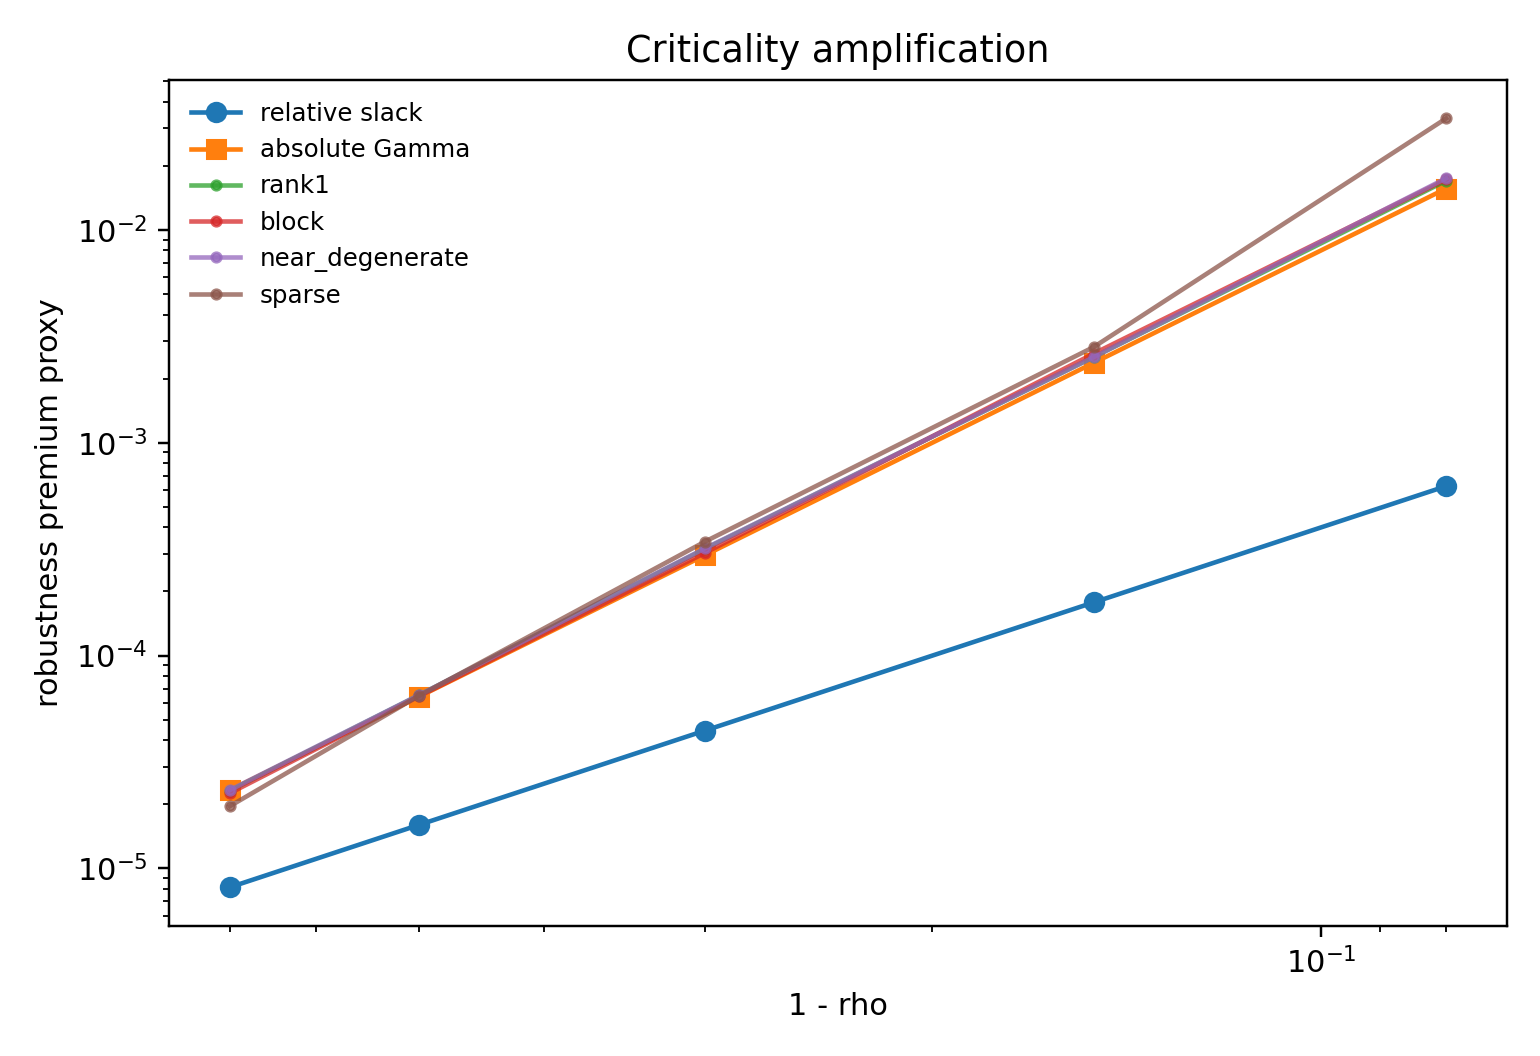
\includegraphics[width=.72\linewidth]{../results/figures/criticality_scaling.png}
\caption{Relative-slack, absolute-Gamma, and matrix-resolvent criticality
amplification.}
\end{figure}

We also run a targeted spectral-gap/visibility ablation using a two-mode
branching matrix with eigenvalues $\rho$ and $1-k(1-\rho)$ for
$k\in\{2,4,8\}$. Perron-visible loadings under a Perron-aligned adversary
recover slope $-2.00$ with median normalized premium ratio $2.8125$. A weak
Perron-visible loading has the same exponent after visibility normalization,
while a Perron-orthogonal loading has no positive Perron-aligned premium. If
the adversary instead moves the second eigenmode, the orthogonal loading again
has slope $-2.00$ when the second mode is near critical; for weakly visible
loadings the median normalized second-mode coefficient falls from $2.639$ at
$k=2$ to $0.0365$ at $k=8$. Thus the lower-bound statement needs both Perron
visibility and an ambiguity set that activates the Perron direction; otherwise
the leading coefficient can vanish or shift to a different near-critical mode.

\begin{figure}[htbp]
\centering
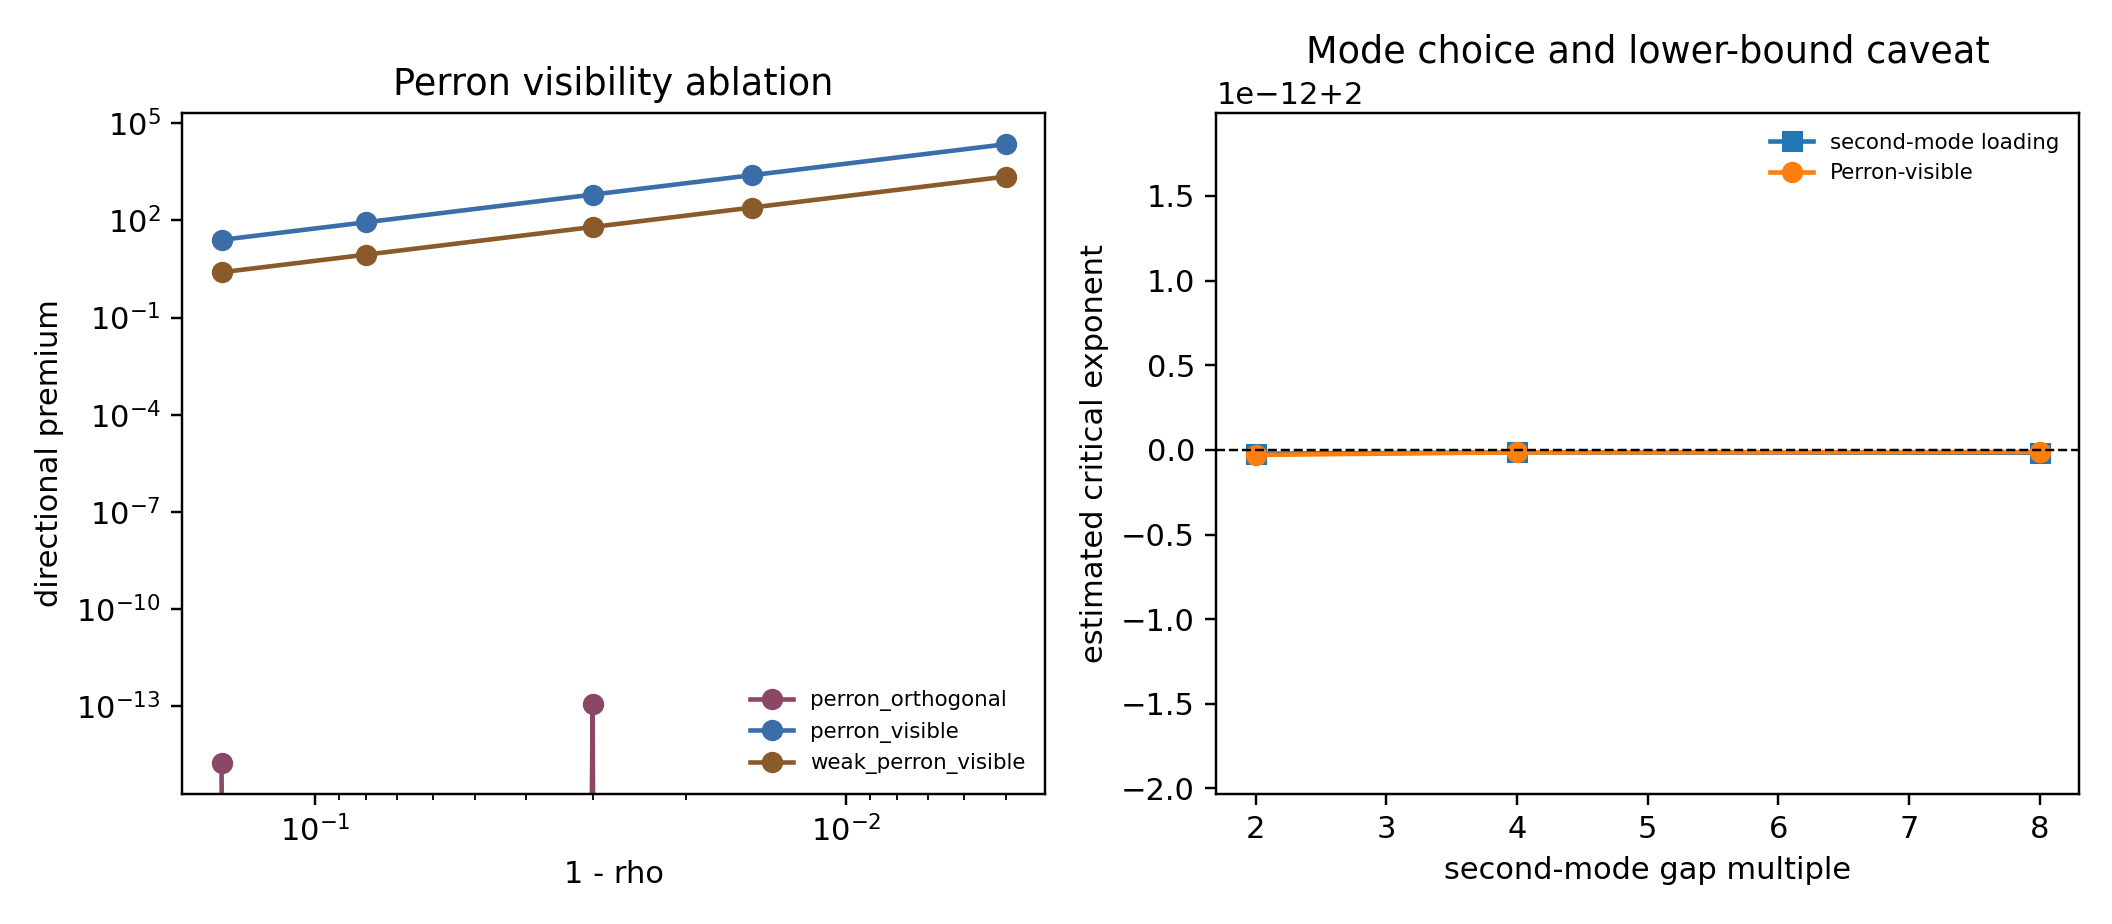
\includegraphics[width=.76\linewidth]{../results/figures/spectral_gap_ablation.png}
\caption{Spectral-gap and Perron-visibility ablation. Perron-visible loadings
recover the square law under aligned ambiguity, while orthogonal loadings only
respond to second-mode perturbations.}
\end{figure}

\subsection{Policy Ablations}

\begin{table}[htbp]
\centering
\small
\begin{tabular}{@{}lrrr@{}}
\toprule
Policy & Certainty equivalent & CVaR5 & Mean diff vs nominal \\
\midrule
robust\_gamma & -13.944 & -38.073 & 0.012 \\
robust\_vol\_only & -13.956 & -38.087 & 0.000 \\
nominal\_hawkes & -13.956 & -38.087 & baseline \\
robust\_gamma\_abs & -13.624 & -37.321 & 0.306 \\
known\_true\_gamma\_no\_ambiguity & -13.952 & -38.082 & 0.004 \\
as\_poisson & -13.974 & -38.113 & -0.017 \\
liquidity\_guard & -13.624 & -37.321 & 0.306 \\
\bottomrule
\end{tabular}
\caption{Common-random-number policy ablation.}
\end{table}

The absolute-Gamma and liquidity-guard policies deliver the strongest displayed
certainty equivalent, CVaR5, and paired mean-wealth differences in the main ablation.
The relative-slack robust-Gamma policy is closer to nominal, with a smaller but
positive paired mean-wealth difference. We do not interpret the
known-true-$\Gamma$ benchmark as an oracle optimum: it is given the stressed
$\rho$, but it does not carry an ambiguity premium, so it under-hedges model
risk in this stress design. The table is best read as evidence that the policy
response depends materially on the ambiguity normalization and on the
withdrawal rule.

\subsection{Policy Time-Step Audit}

Because the simulator validation below shows that near-critical Hawkes counts
are sensitive to bin width, we reran focused policy comparisons at
$\Delta t\in\{0.04,0.02,0.01\}$ for the stressed $\epsilon=0.02$,
$\hat\rho=0.92$ scenario. Across the tested time steps, the relative-slack
robust-Gamma policy keeps a positive mean-wealth advantage over nominal Hawkes:
$0.042$--$0.060$. The absolute-Gamma policy produces much larger mean-wealth
gains, $1.154$--$1.366$, but with negative lower paired quantiles, consistent
with the broader point that ambiguity normalization changes the economic
policy, not only the scale of the premium.

\begin{figure}[htbp]
\centering
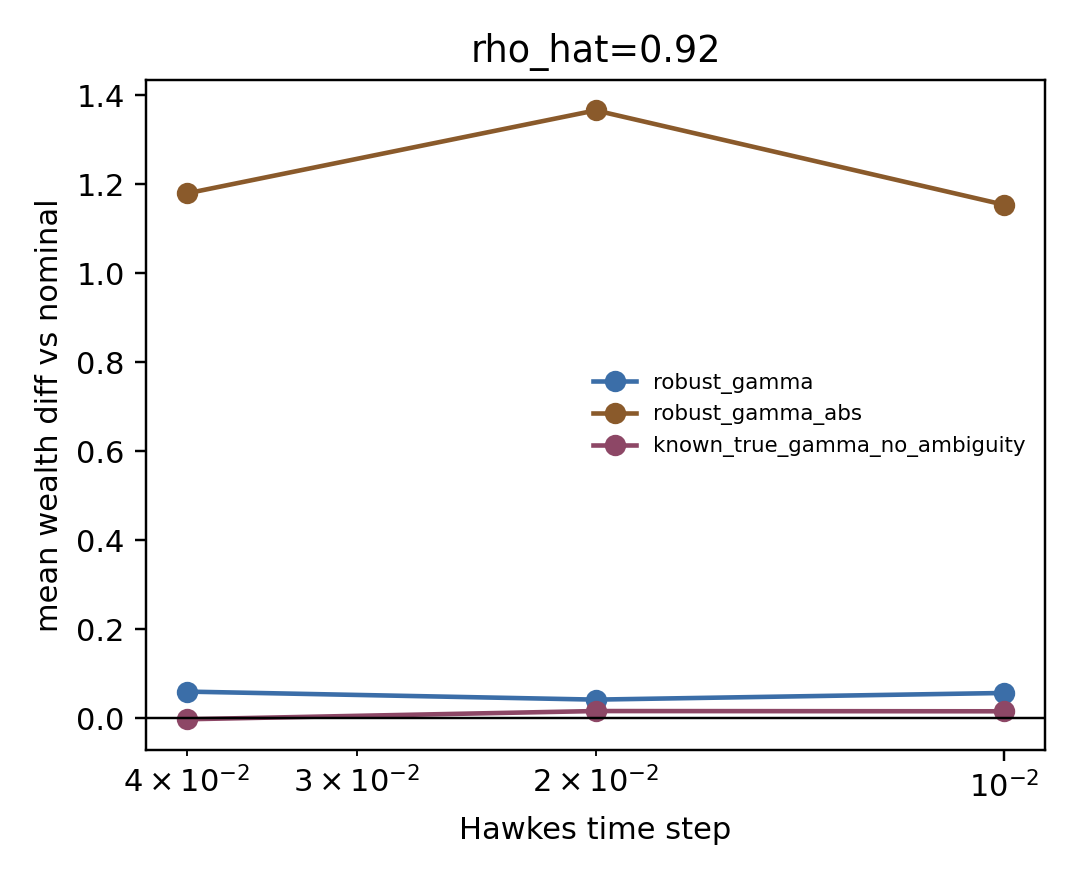
\includegraphics[width=.76\linewidth]{../results/figures/policy_dt_convergence.png}
\caption{Focused policy time-step audit. Positive values indicate outperformance
relative to nominal Hawkes on the same scenario.}
\end{figure}

\subsection{Ogata Arrival Audit}

We also compare the fast binned Hawkes recursion against event times generated
by Ogata thinning and then binned onto the same decision grid. In the
$\epsilon=0.02$, $\hat\rho=0.92$ check, the discrete recursion produces more
events than the Ogata reference: mean total events are $226.8$ under the
discrete recursion and $185.5$ under Ogata-binned arrivals. The relative-slack
robust-Gamma policy is positive relative to nominal under discrete arrivals,
with mean-wealth advantage $0.030$, but is essentially flat and slightly
negative under Ogata-binned arrivals, with mean-wealth difference $-0.001$.
Absolute-Gamma remains strongly positive under both generators, with advantages
$0.705$ and $0.690$. This check weakens any blanket claim that robust-Gamma
dominates under every arrival generator, while still showing that the
binned-recursion result is not wildly disconnected from an event-time reference.

\begin{figure}[htbp]
\centering
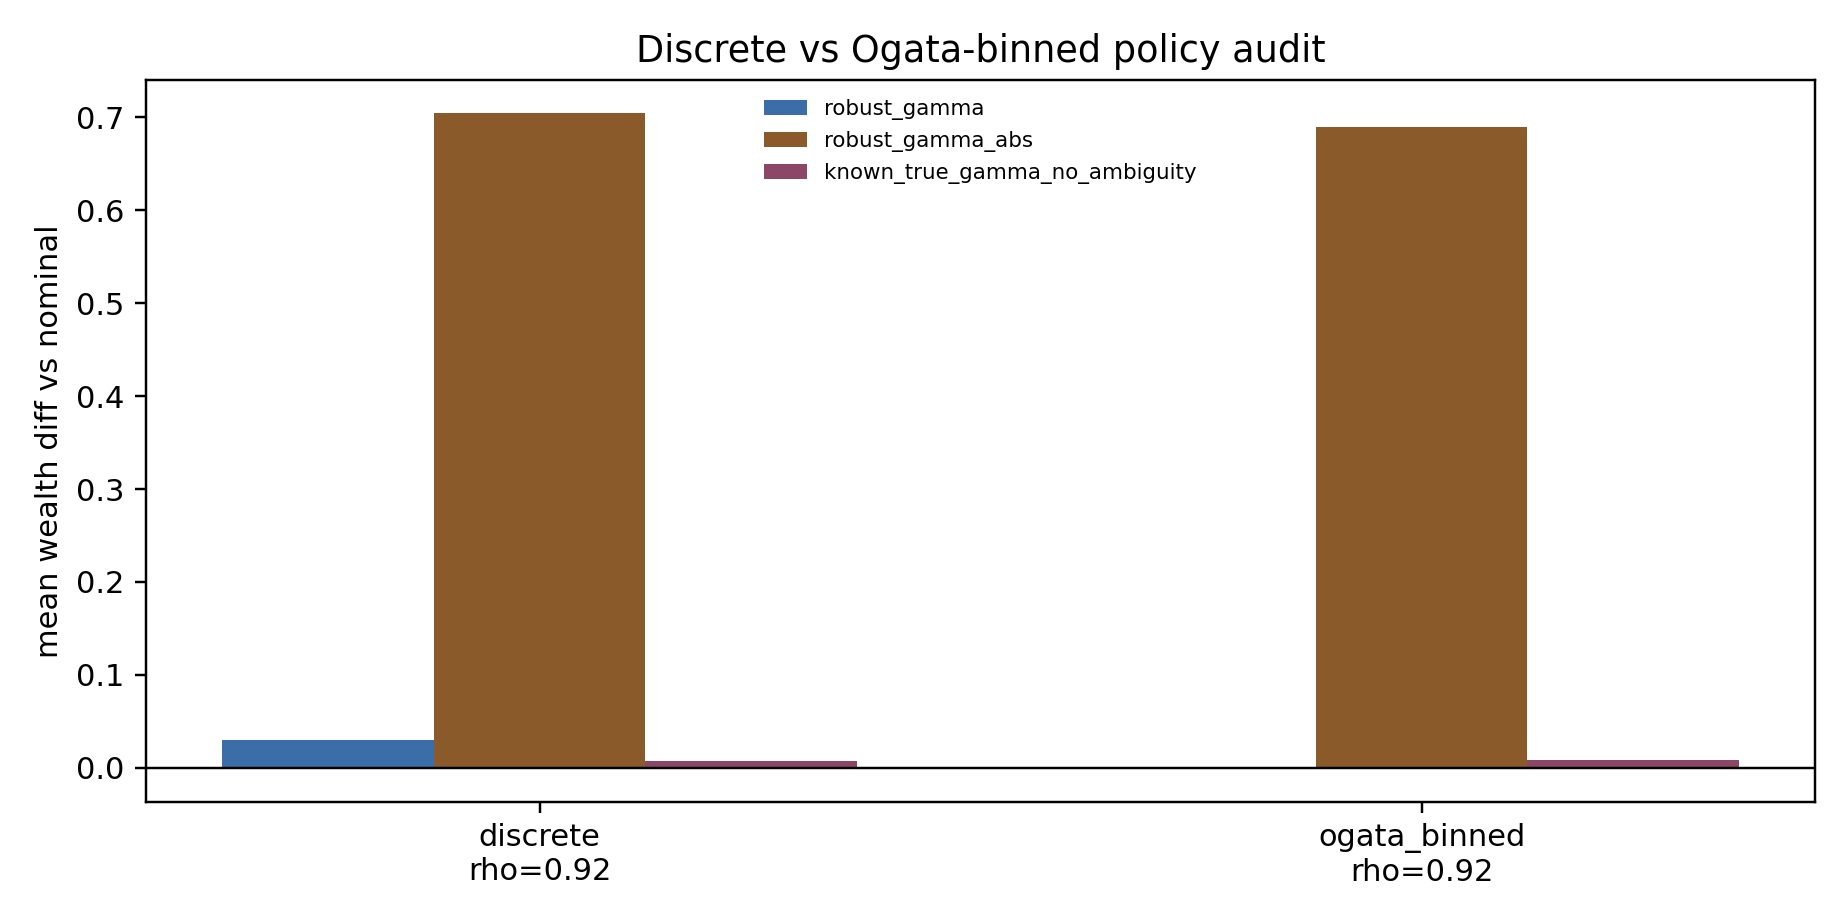
\includegraphics[width=.76\linewidth]{../results/figures/policy_ogata_audit.png}
\caption{Focused policy audit under fast discrete arrivals and Ogata-binned
event arrivals for $\hat\rho=0.92$.}
\end{figure}

\subsection{Event-Queue Backtest}

We then run a reduced event-driven queue backtest on Ogata Hawkes event times.
The evaluator reuses each event path across policies, updates quotes every
$\Delta t=0.02$, tracks a simple queue-ahead state, and records side-time spent
not quoting. For $\hat\rho=0.92$ over 24 paths, robust-Gamma is nearly flat but
positive relative to nominal, with mean-wealth difference $0.0125$, while
absolute-Gamma and the liquidity guard each improve mean wealth by $0.342$. In
this reduced run, fill rates are identical across policies at $0.943$, the
side-time no-quote fraction is $0.064$, and the full no-quote time fraction is
zero. The result is not a production queue simulator, but it provides an
event-time execution stress test for the checked regime.

\begin{figure}[htbp]
\centering
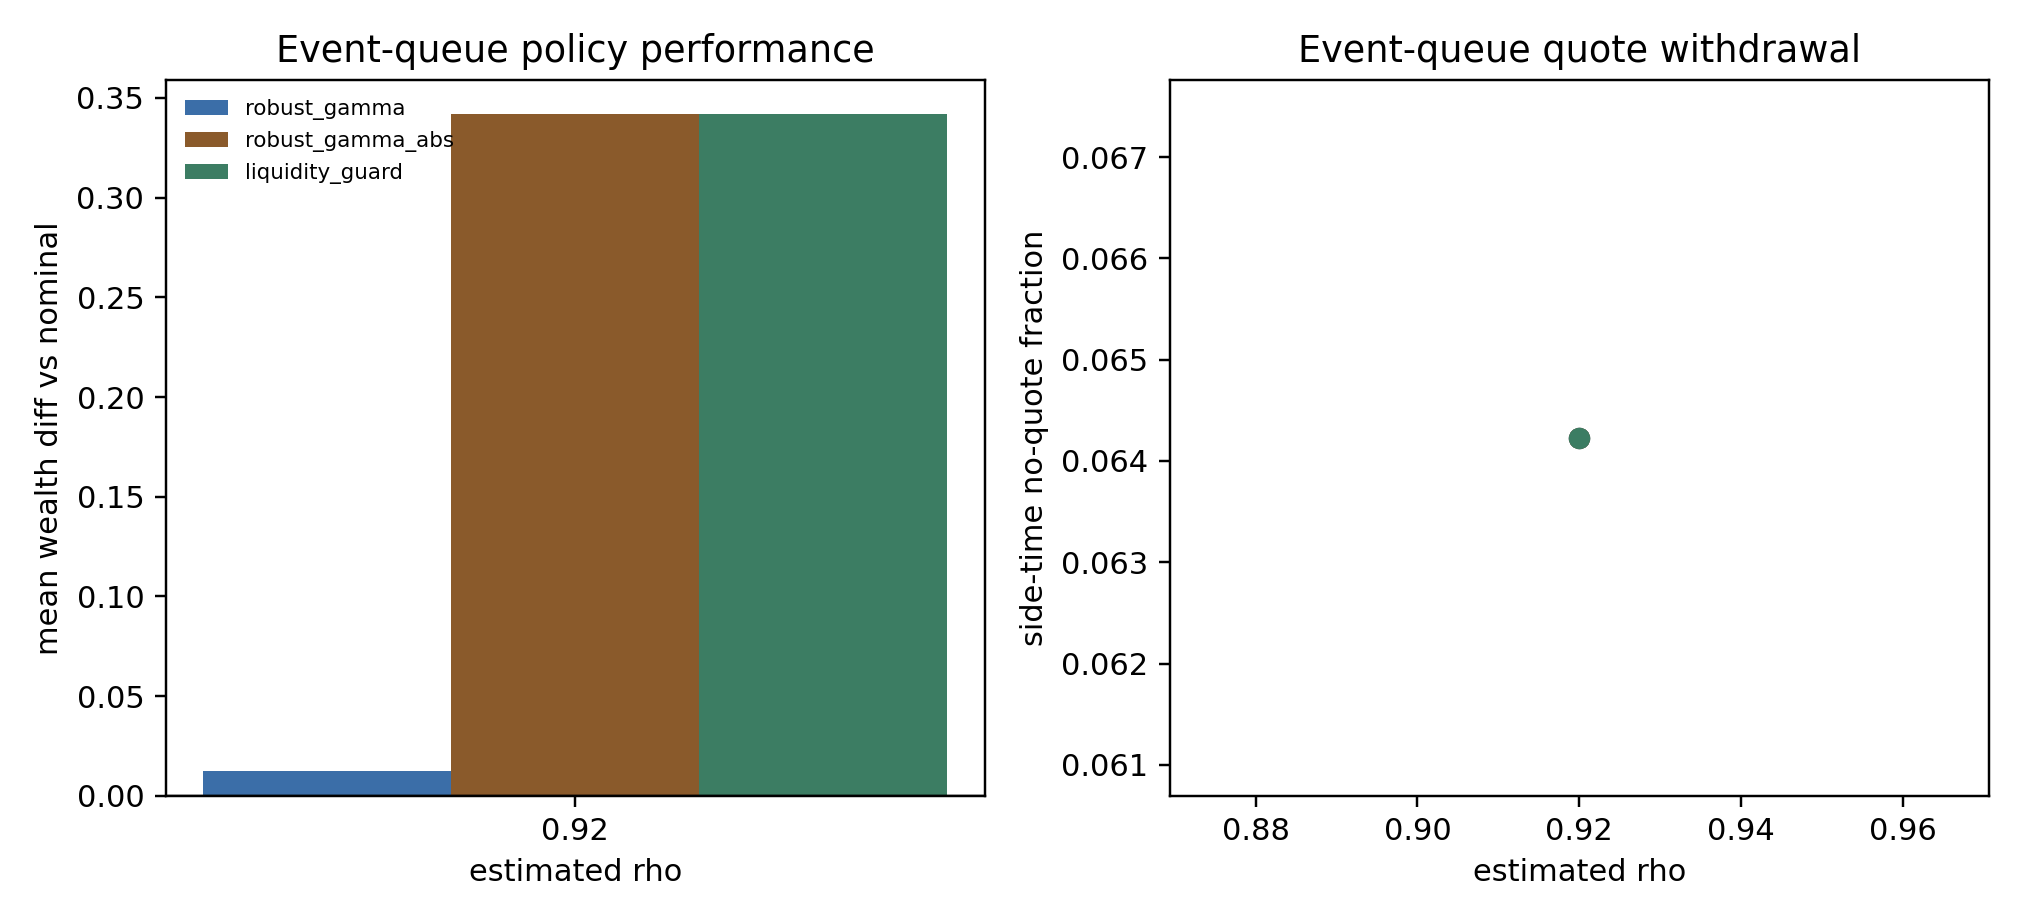
\includegraphics[width=.76\linewidth]{../results/figures/event_queue_backtest.png}
\caption{Reduced event-queue policy performance and shared side-time no-quote fraction.}
\end{figure}

\subsection{Public LOBSTER Top-Of-Book Replay}

As a public-data execution check, we replay the policy family on actual LOBSTER
message/order-book streams. The replay uses the first 80,000 synchronized
messages per ticker, posts active policies at the displayed L1 quotes subject
to an inventory cap, depletes a simple queue-ahead proxy using observed
execution sizes, and marks to the observed midprice. Under the calibrated
side-aware spectral radii, all tested policies remain inside the L1 activity
threshold, so the replay intentionally reports no artificial separation: mean
terminal wealth is $341.691$, mean fills are $3071.8$, and side-time no-quote
share is $0.198$ for each policy. Under the near-critical stress setting
$\hat\rho=0.97$, nominal and relative-slack robust-Gamma remain active on the
same real event streams, while absolute-Gamma and the liquidity guard fully
withdraw: their mean wealth difference versus nominal is $-341.691$, mean
fills are zero, and side-time no-quote share is one. This is not a production
queue simulator, but it shows that the quote-withdrawal transition can be
replayed on real event paths and L1 prices.

We also run an offset-aware L1 replay. It converts each policy's continuous
offsets into visible quote states: join the displayed best quote, improve
inside the spread, rest away from L1, or withdraw. Away quotes are not filled,
because one-level data cannot identify hidden depth. Under calibrated
side-aware spectral radii, tick rounding still makes policy PnL coincide, but
the replay explains the quote placement: mean side-time is $0.024$ joining,
$0.428$ improving, $0.448$ away from L1, and $0.101$ withdrawn. Under
$\hat\rho=0.97$, absolute-Gamma and the liquidity guard fully withdraw. This
is a stronger public-data audit than the binary replay, while still stopping
short of production execution claims.

Finally, we run a displayed-depth replay on the uniform level-10 LOBSTER panel.
This removes the one-level limitation for away quotes: if a rounded quote price
rests inside the displayed ten-level ladder, the replay initializes queue-ahead
from all better displayed levels plus a same-level queue fraction, and observed
executions and visible depth changes can deplete that queue. Under calibrated
side-aware spectral radii, policies still coincide after tick rounding, but the
state mix is more informative: mean side-time is $0.018$ joining L1, $0.428$
improving, $0.408$ resting at visible depth, and $0.146$ withdrawn, with mean
visible depth rank $2.431$ and mean fills $1420.2$. Under $\hat\rho=0.97$,
absolute-Gamma and the liquidity guard fully withdraw, with mean wealth
difference $-120.216$ versus nominal. The replay remains conservative about
hidden liquidity and exact priority, but it is no longer L1-only.

As a stricter execution audit, we add a priority-aware level-10 replay. At each
quote reset, the synthetic order is placed behind the full displayed size at
the same price, later same-price limit orders are tracked by order identifier
as being behind the synthetic quote, and cancellations/executions of those
behind orders are not allowed to deplete our queue position. Queued fills are
credited only from residual same-price execution volume after displayed queue
ahead has been depleted; exact queue exhaustion with no residual volume is
recorded but not filled, and partial fills are credited by residual lots. Under
calibrated side-aware spectral radii, this stricter replay exposes how much of
the displayed-depth result relied on a heuristic same-level queue cap: mean fill
events are $21.6$ but mean filled lots are only $15.53$, mean terminal wealth is
$-7.839$, and mean side-time is $0.019$ joining L1, $0.530$ improving,
$0.422$ resting at visible depth, and $0.029$ withdrawn. Under
$\hat\rho=0.97$, absolute-Gamma and liquidity-guard policies fully withdraw
and avoid the nominal priority-replay loss, giving mean wealth difference
$+5.964$ versus nominal. The regenerated artifact also records queue-position
invariants: in the calibrated baseline, mean initial displayed queue ahead is
$62.03$ lots across $1810.4$ visible quote resets, queued fills average $1.2$,
inside-spread improve fills average $20.4$, partial-fill events average $7.6$,
the maximum zero-residual prevented-fill count is $1$, and the maximum
queue-violation count is zero. This is the closest public-data replay in the
package to queue-position accounting; it still cannot observe hidden liquidity
or recover order identifiers for anonymous queue ahead present before the
synthetic quote arrives.

As a depth supplement, we also replay the deepest public LOBSTER files available
for the sample panel: level-50 AAPL and MSFT on their shorter one-hour public
window. This supplement uses all $50$ displayed levels in those files and
records mean fill events $23.0$, mean filled lots $16.82$, mean queued fills
$2.5$, mean improve fills $20.5$, mean partial-fill events $8.0$, max visible
depth rank $5$, and maximum queue-violation count zero. Because only two tickers
have public level-50 samples in the mirror, this is a supplement rather than the
headline five-ticker panel.

We also run a priority-assumption sensitivity grid for the nominal policy. The
grid varies the fraction of displayed same-price queue placed ahead of the
synthetic order over $\{0,0.5,1\}$ and a queue-stress multiplier over
$\{1,1.5,2\}$. The multiplier is applied to the public displayed queue-ahead
proxy as a conservative stress test; it is not evidence that hidden depth has
been observed. On the calibrated level-10 panel, the optimistic displayed
priority setting $(0,1)$ gives mean filled lots $16.53$; the strict
displayed-priority baseline $(1,1)$ gives mean filled lots $15.53$; and the
most conservative tested queue-stress setting $(1,2)$ gives mean filled lots
$14.87$. The small numerical range is a negative but useful empirical result:
public displayed books rarely identify enough residual same-price execution
volume to make hidden-priority assumptions strongly estimable. Across the
sensitivity grid, the maximum queue-violation count remains zero.

As a final queue-audit layer, we reconstruct the observable level-10 book from
messages and compare it to the official LOBSTER snapshots. The reconstructor
starts from the first official snapshot, tracks all post-start order IDs, and
re-anchors every 100 messages to measure local reconstruction quality rather
than all-day truncation drift. Across 399,995 processed events and 40,000
compared snapshots, panel mean top-of-book price match is $0.9997$, full
10-level price match is $0.9376$, top-of-book size MAE is $0.056$ shares, and
full-depth size MAE is $38.1$ shares. This supports local near-touch priority
analysis from public messages while keeping deeper queue-position claims
conservative.

\begin{figure}[htbp]
\centering
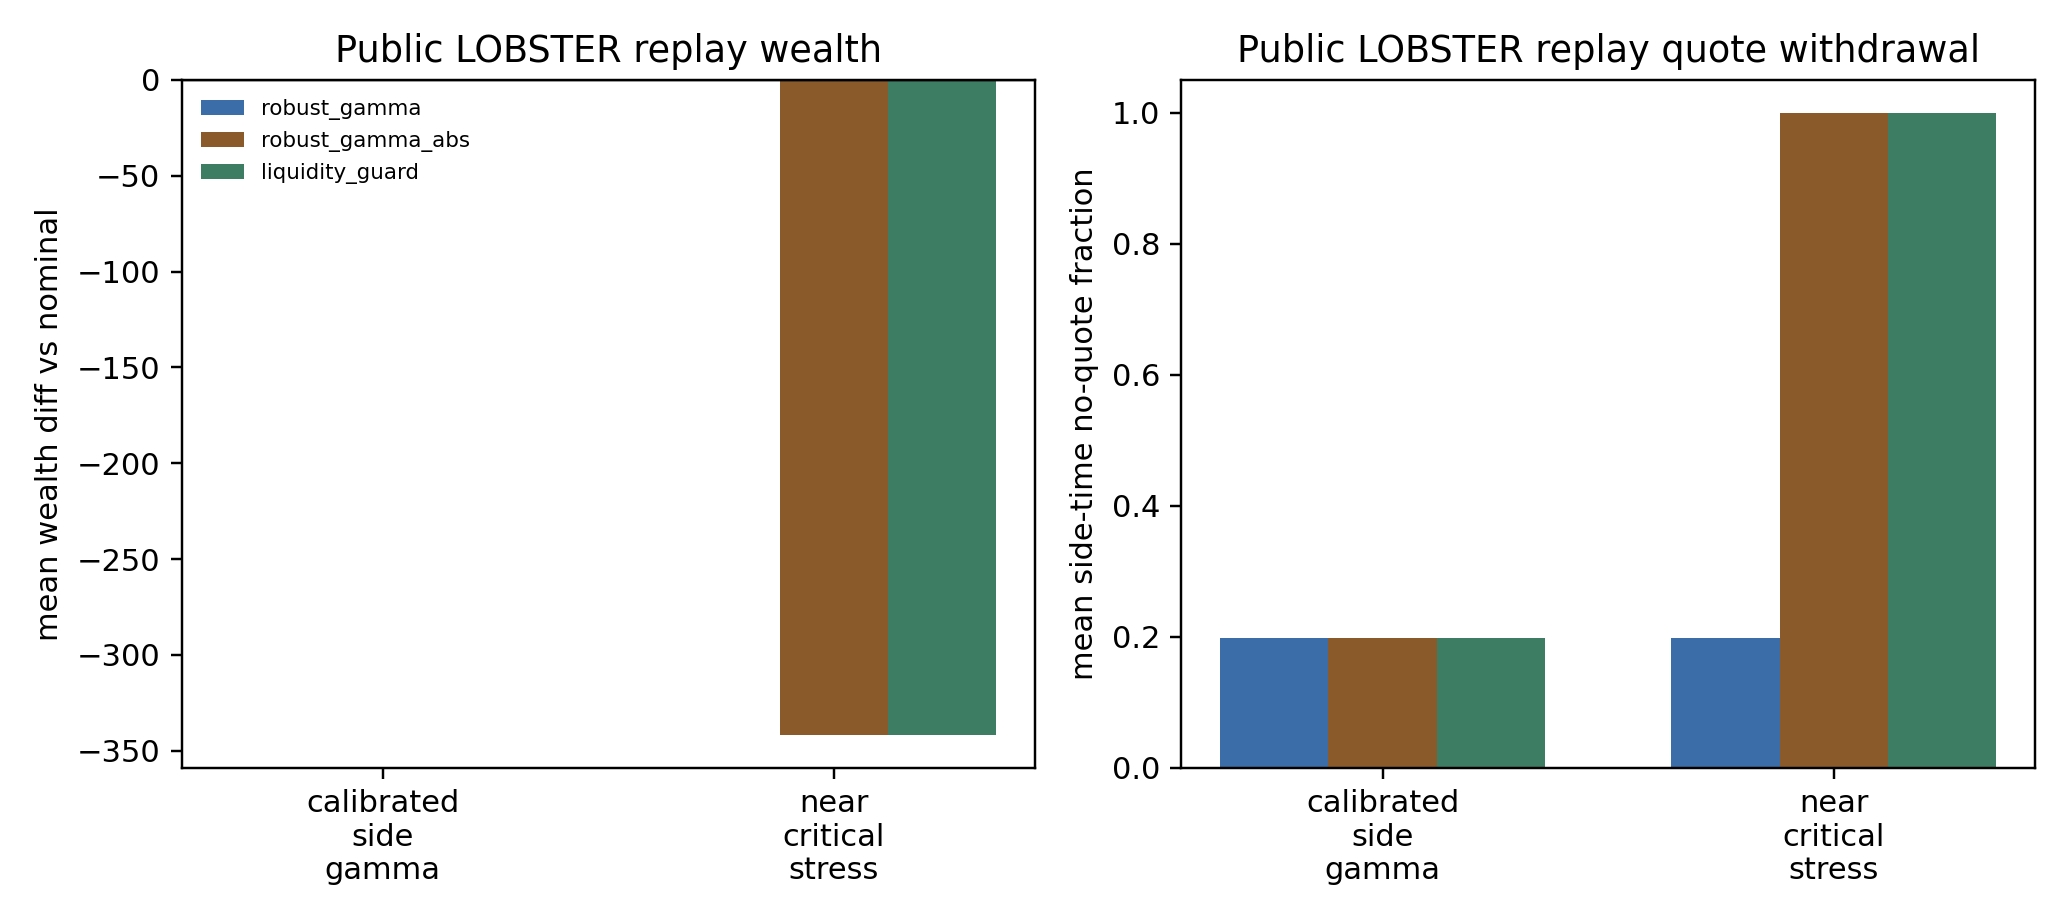
\includegraphics[width=.78\linewidth]{../results/figures/lobster_top_of_book_replay.png}
\caption{Public LOBSTER top-of-book replay on actual message/order-book
streams. The binary top-of-book rule makes calibrated policies coincide, while
near-critical absolute-Gamma ambiguity forces quote withdrawal on the same
data paths.}
\end{figure}

\begin{figure}[htbp]
\centering
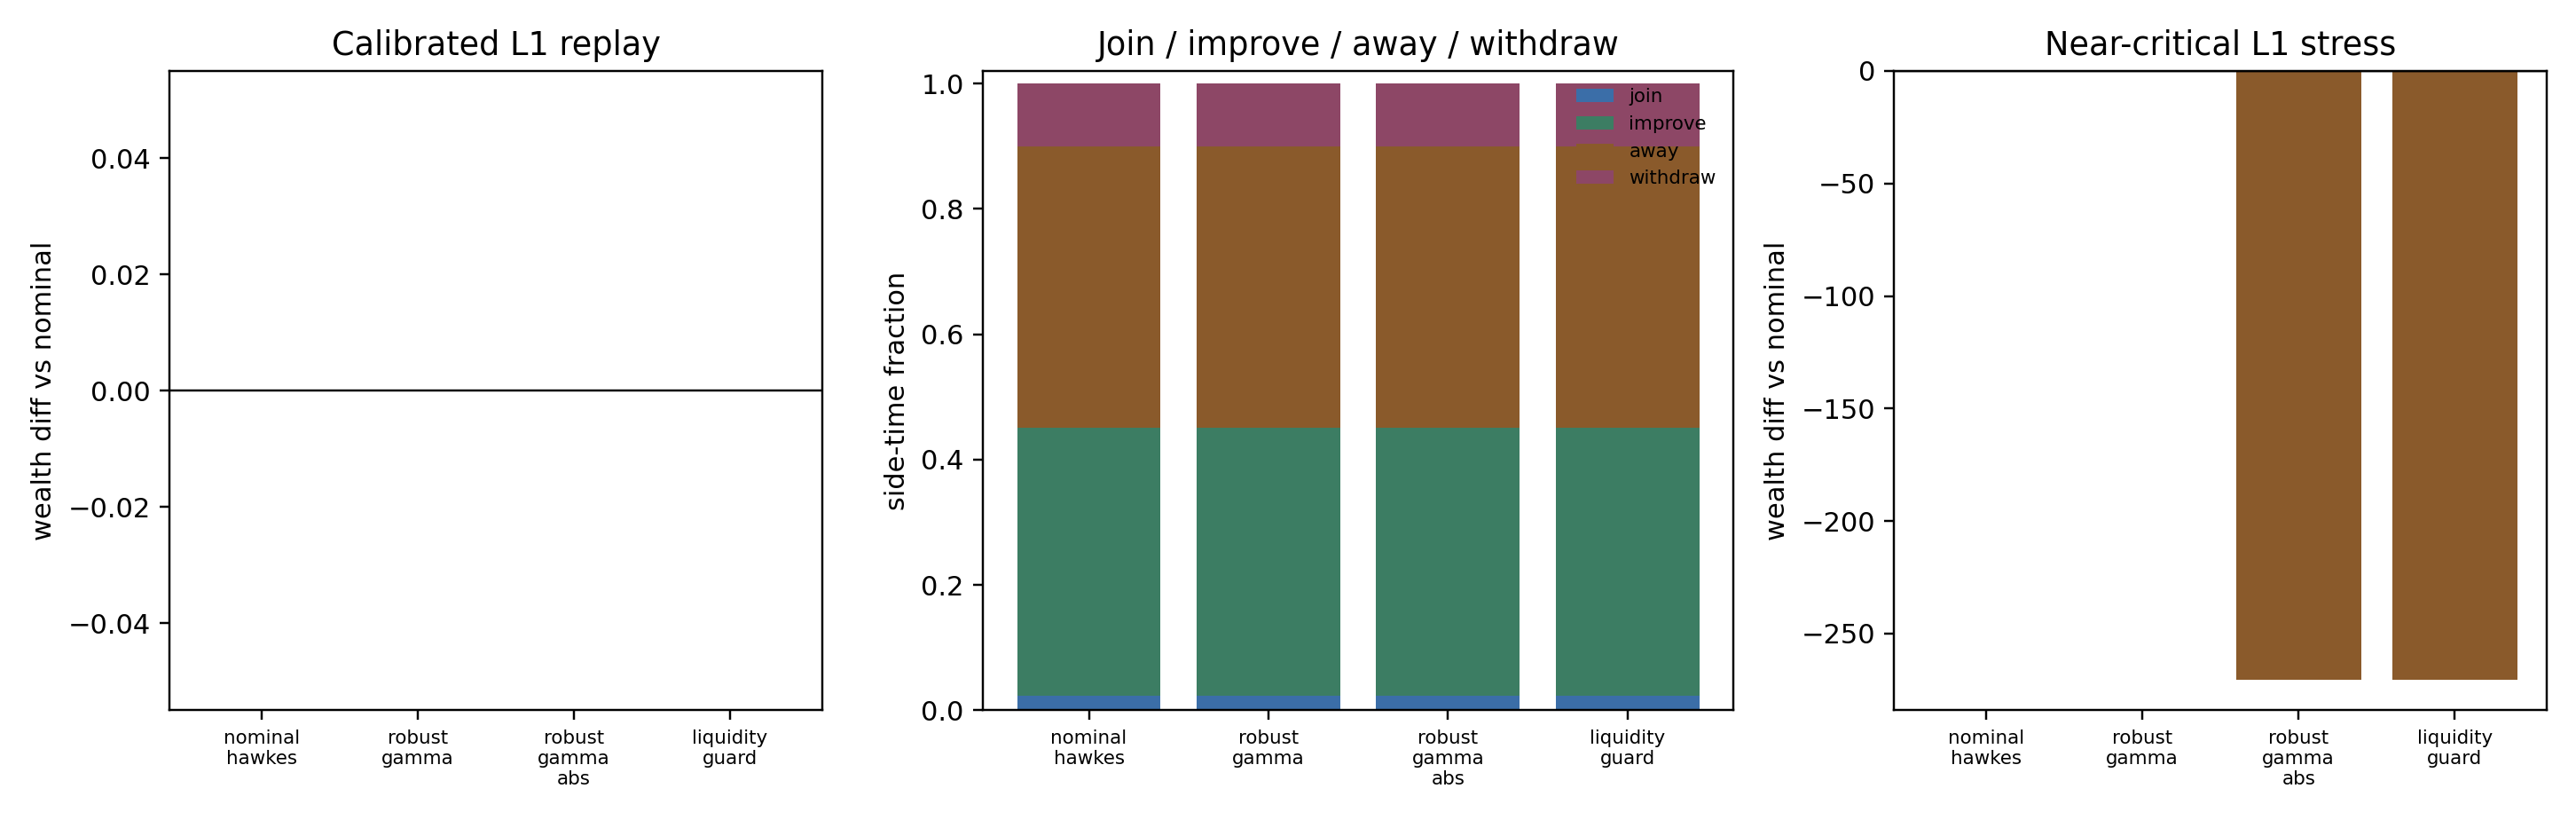
\includegraphics[width=.86\linewidth]{../results/figures/lobster_l1_quote_replay.png}
\caption{Offset-aware L1 quote replay. The calibrated public sample still does
not separate policy wealth after tick rounding, but it reveals visible quote
state fractions and shows that near-critical absolute-Gamma ambiguity produces
full withdrawal.}
\end{figure}

\begin{figure}[htbp]
\centering
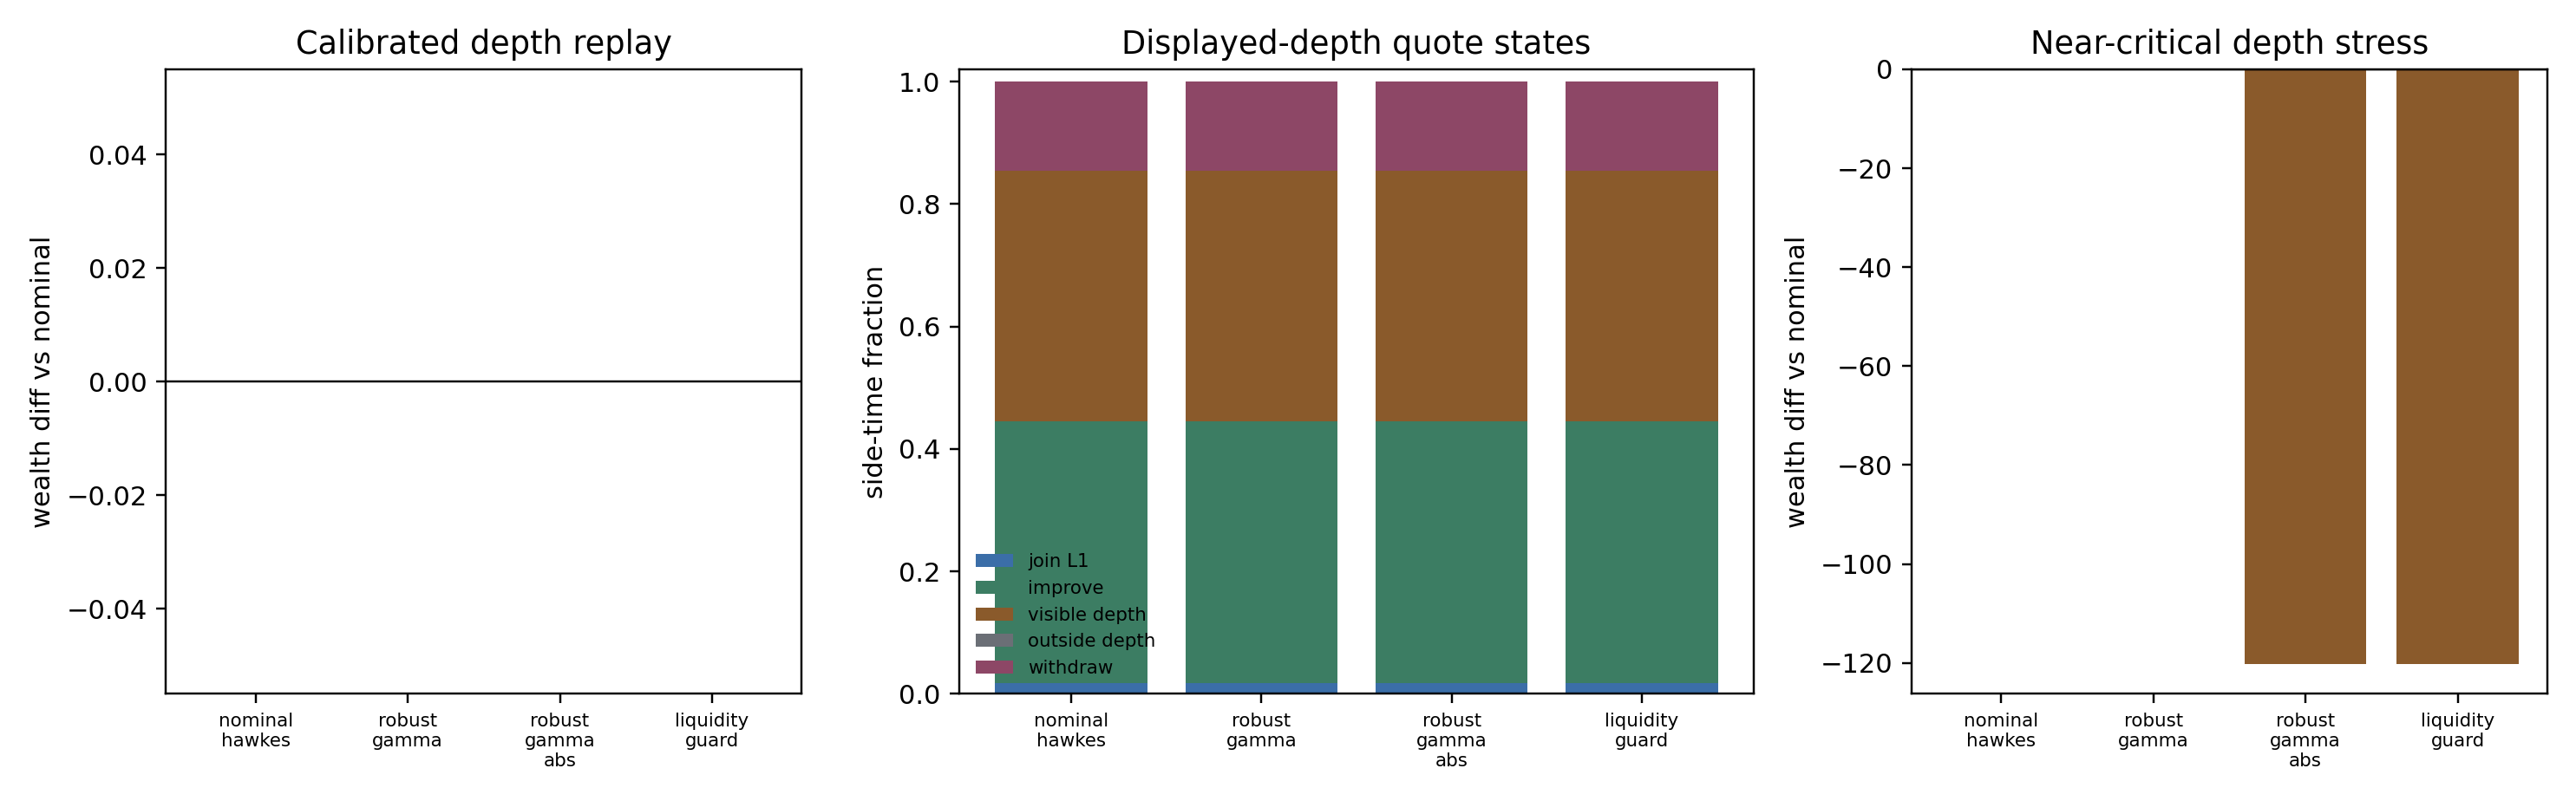
\includegraphics[width=.88\linewidth]{../results/figures/lobster_depth_quote_replay.png}
\caption{Displayed-depth level-10 LOBSTER quote replay. Away-from-L1 quotes can
fill when they rest inside the visible book and observed executions/depth
changes deplete displayed queue ahead.}
\end{figure}

\begin{figure}[htbp]
\centering
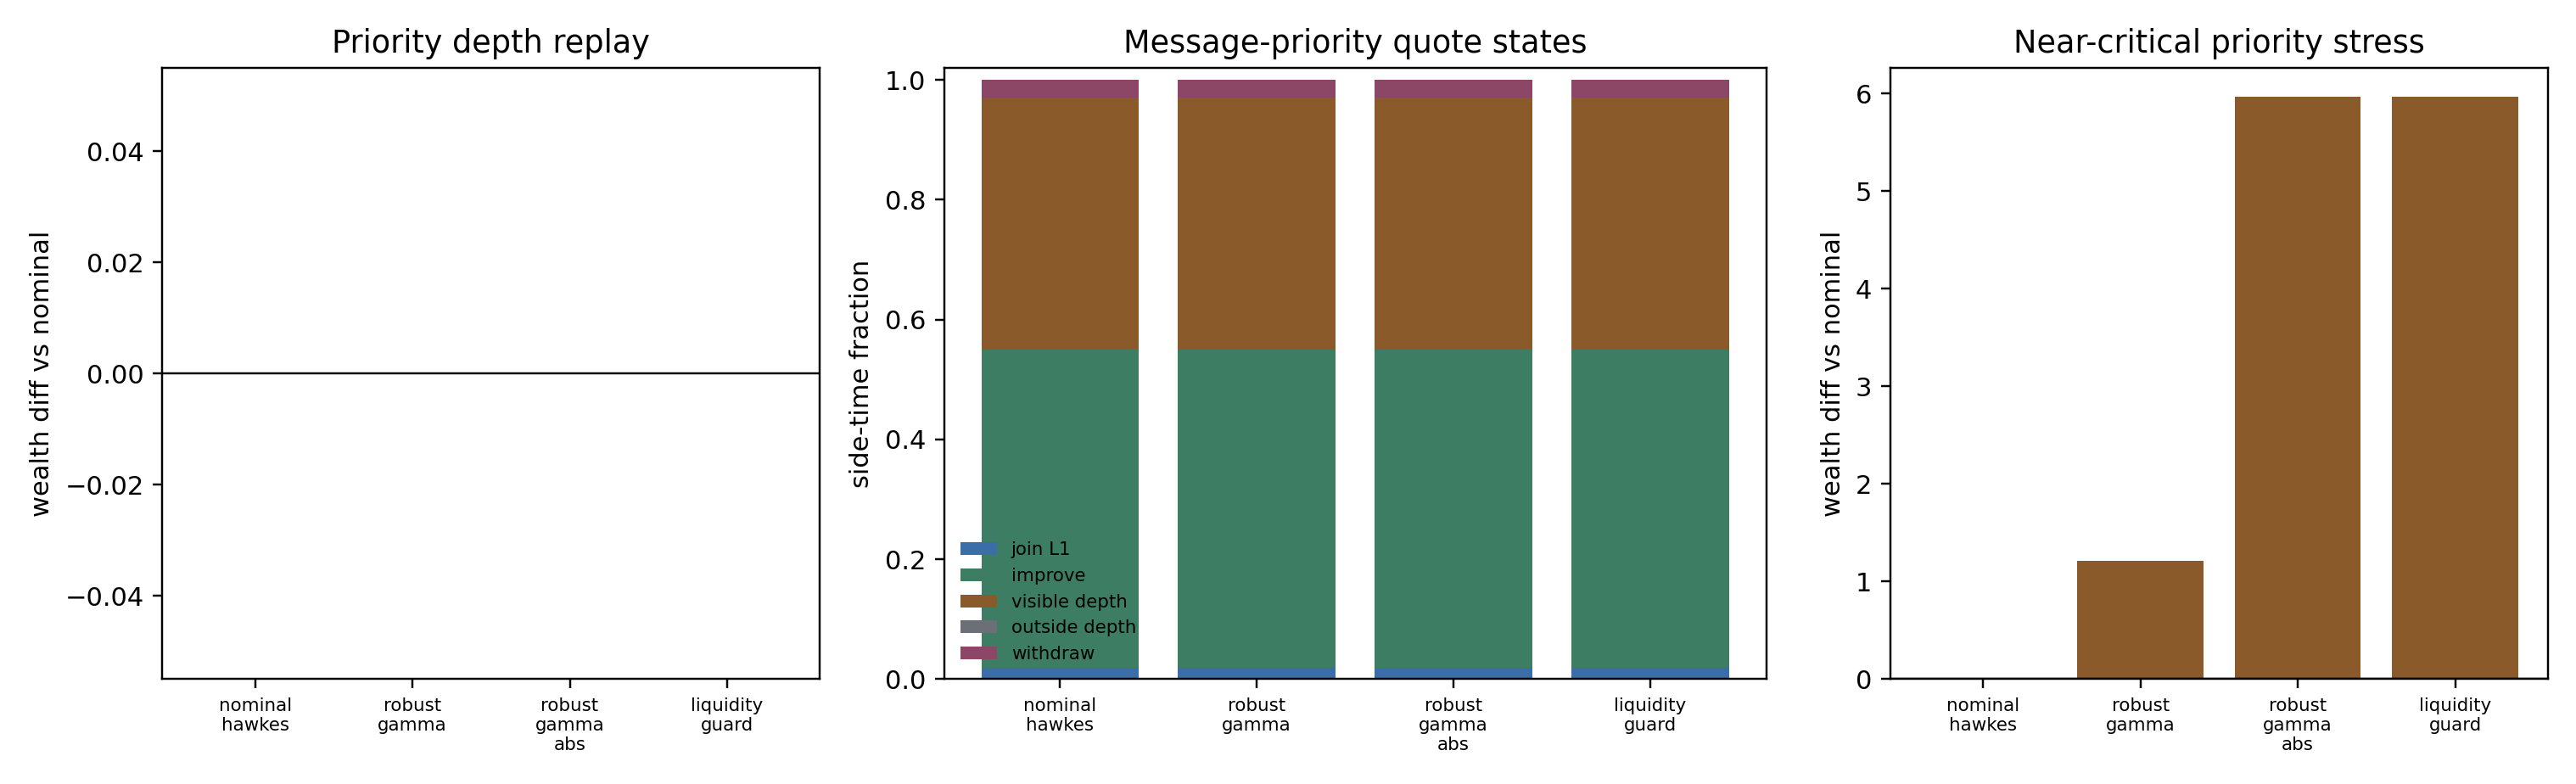
\includegraphics[width=.88\linewidth]{../results/figures/lobster_priority_depth_quote_replay.png}
\caption{Residual-volume priority-aware level-10 LOBSTER quote replay.
Same-price orders arriving after the synthetic quote are tracked behind it,
queued fills require residual execution volume after displayed queue-ahead
depletion, and partial fills are credited by residual lots.}
\end{figure}

\begin{figure}[htbp]
\centering
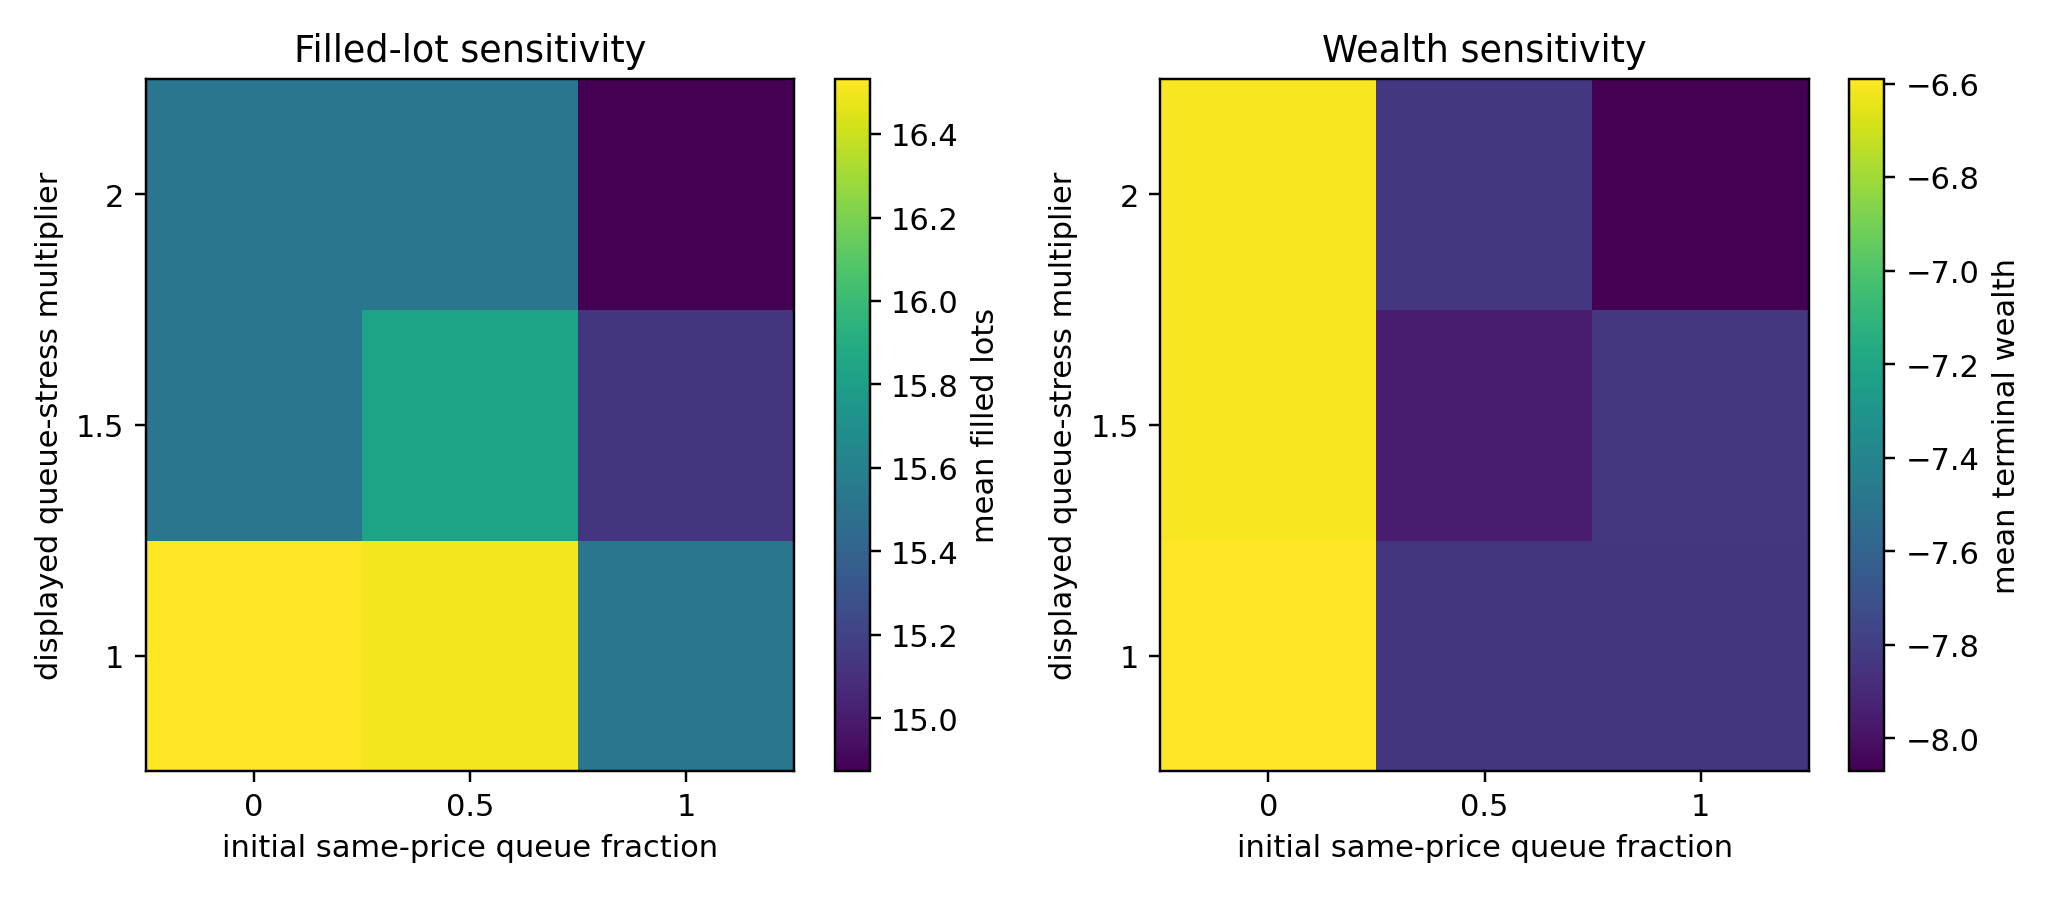
\includegraphics[width=.84\linewidth]{../results/figures/lobster_priority_depth_sensitivity.png}
\caption{Priority-assumption sensitivity for the nominal level-10 replay. The
grid varies initial same-price displayed priority and a displayed queue-stress
multiplier; filled lots remain rare across the grid, exposing the public-data
limit of same-price priority identification.}
\end{figure}

\begin{figure}[htbp]
\centering
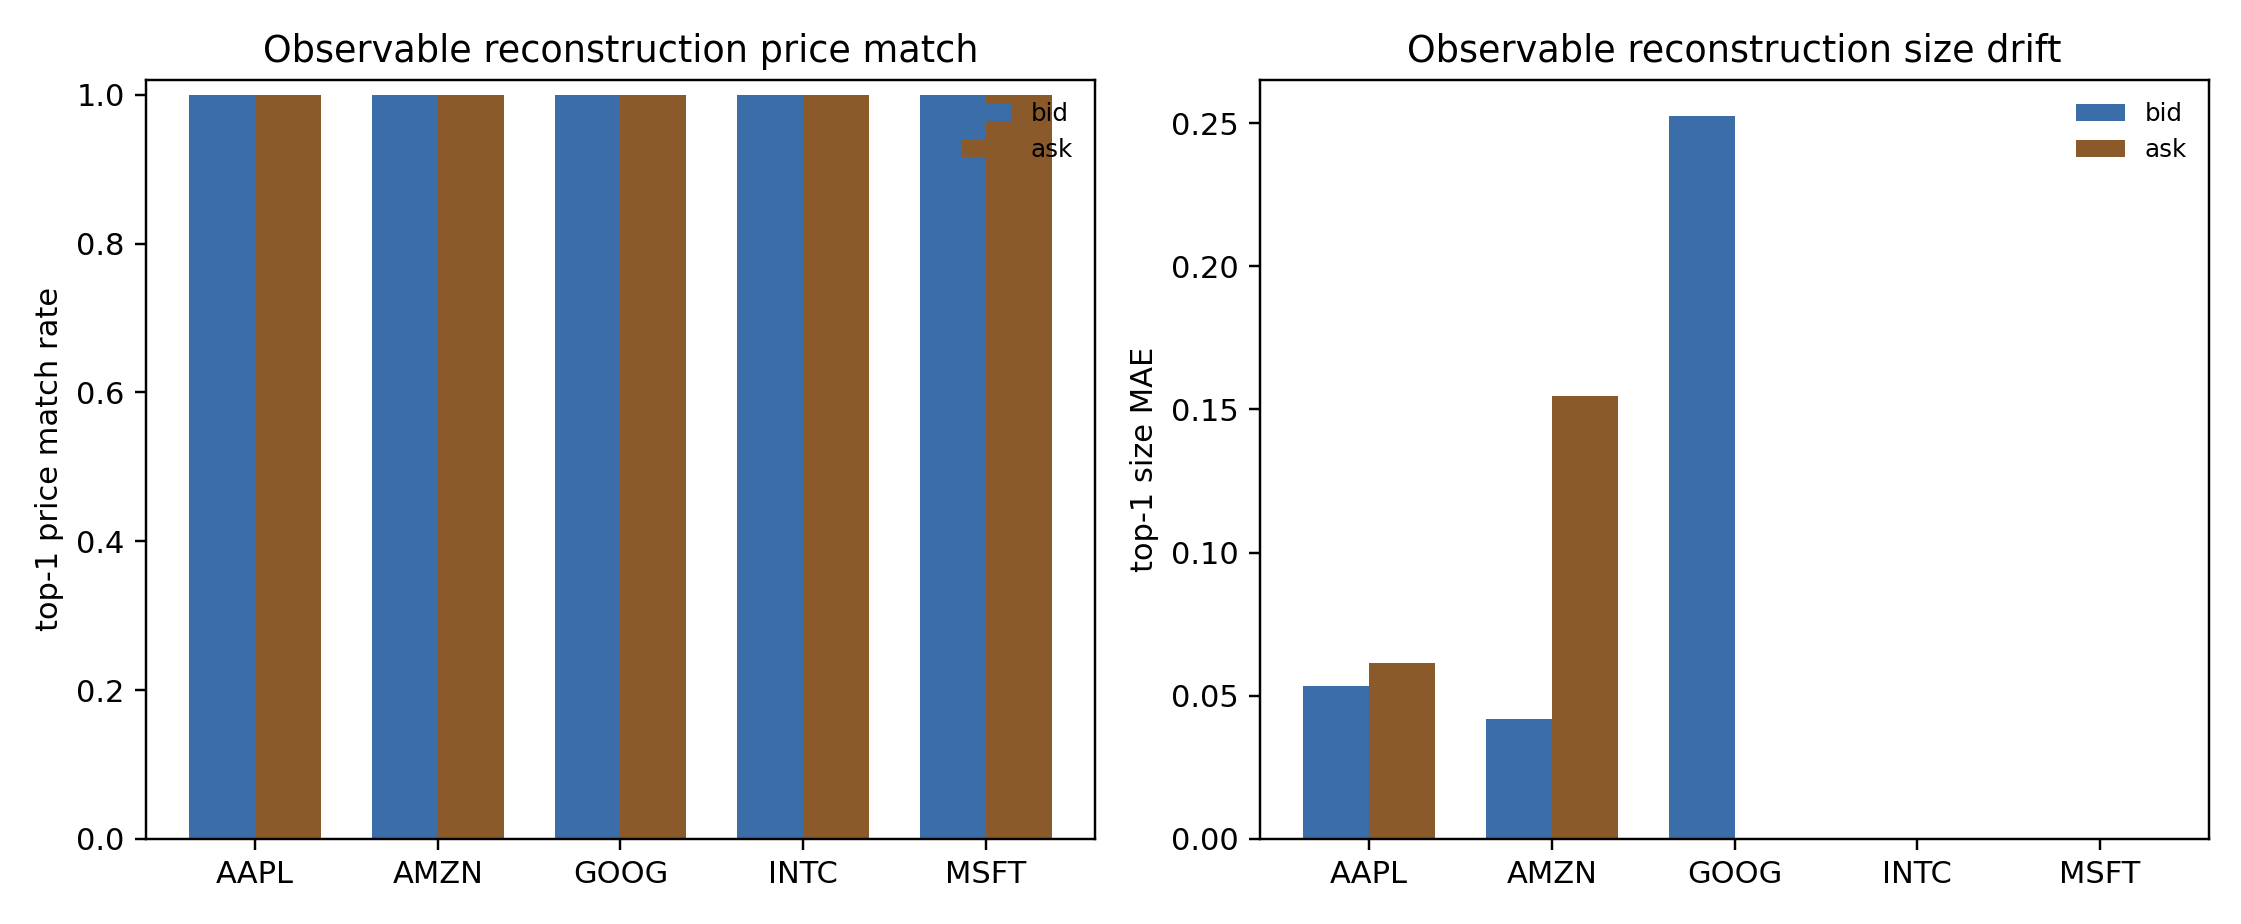
\includegraphics[width=.84\linewidth]{../results/figures/lobster_orderbook_reconstruction.png}
\caption{Observable order-book reconstruction audit. Re-anchored message-level
reconstruction matches top-of-book prices almost exactly, while full-depth size
drift remains visible.}
\end{figure}

\subsection{Simulator Validation}

The slow Ogata reference simulator exposes an important numerical issue. Coarse
time discretization can create spurious critical amplification. At
$\rho=0.90$, the relative mean-count bias drops from $3.15$ at $\Delta t=0.08$
to $0.03$ at $\Delta t=0.01$. At $\rho=0.97$, even $\Delta t=0.005$ leaves
about $0.15$ relative bias in the current short-horizon setting.

\begin{figure}[htbp]
\centering
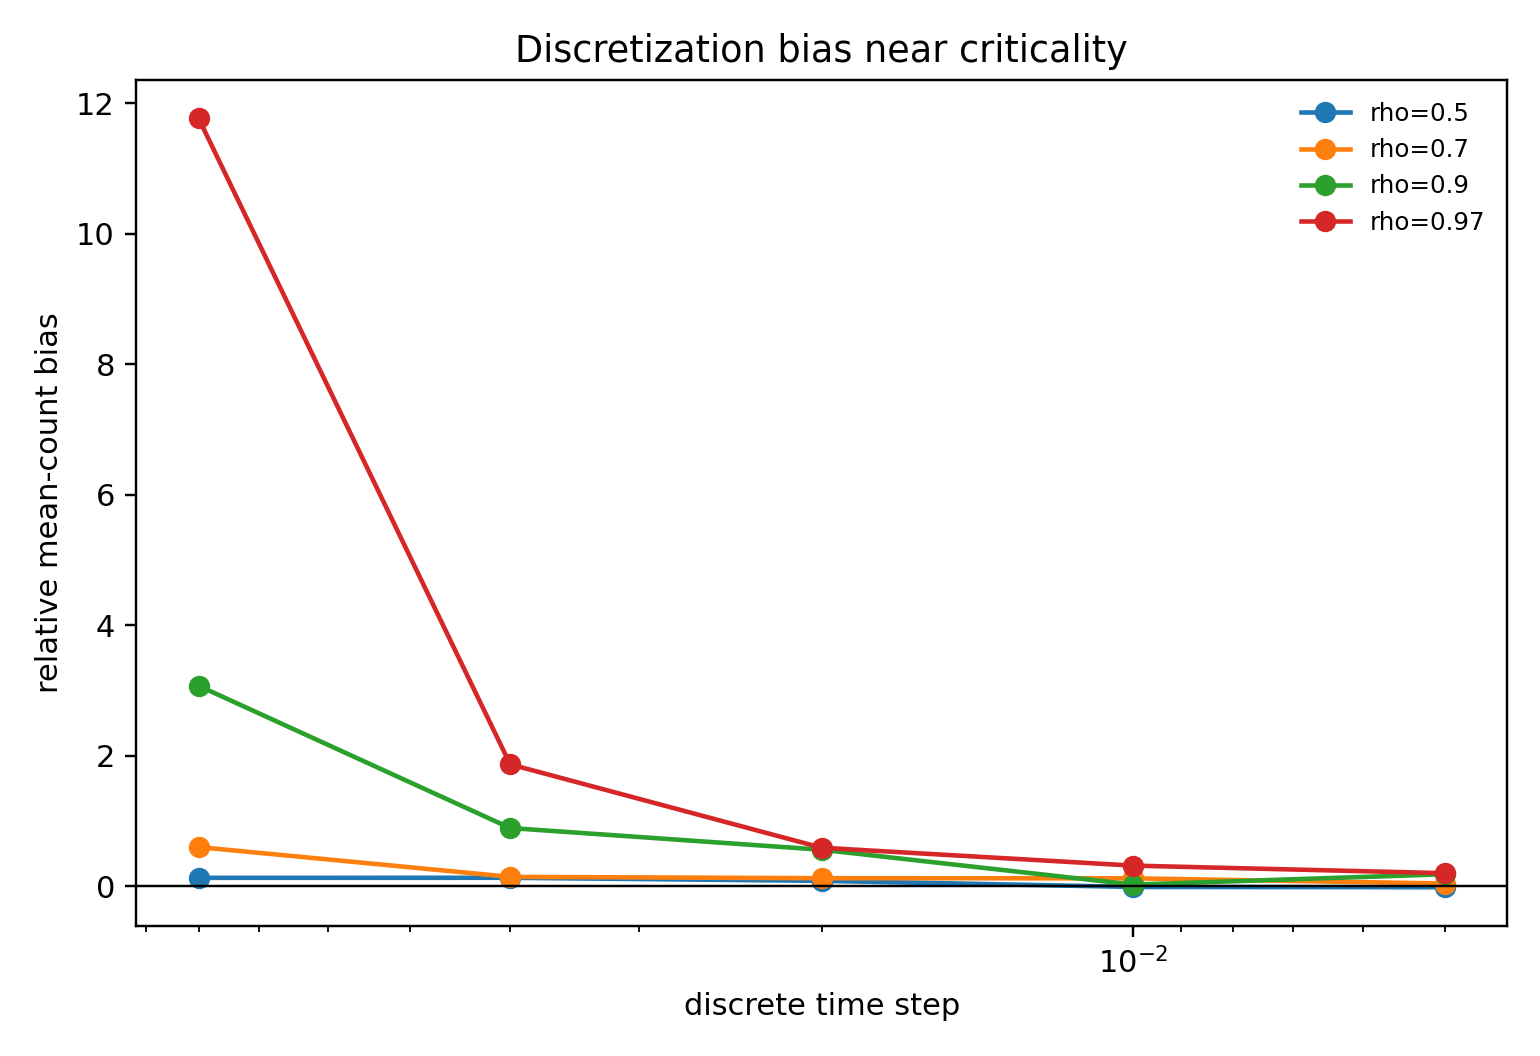
\includegraphics[width=.72\linewidth]{../results/figures/discretization_bias.png}
\caption{Time-discretization bias grows sharply near criticality.}
\end{figure}

\subsection{Calibration Noise}

A simple Fano-based criticality estimator confirms that near-critical
calibration is fragile. For $\rho=0.97$, short horizons under-estimate
criticality, while longer horizons can over-shoot because the count variance is
dominated by rare clusters. This motivates reporting uncertainty intervals for
all empirical $\hat\rho$ estimates.

\begin{figure}[htbp]
\centering
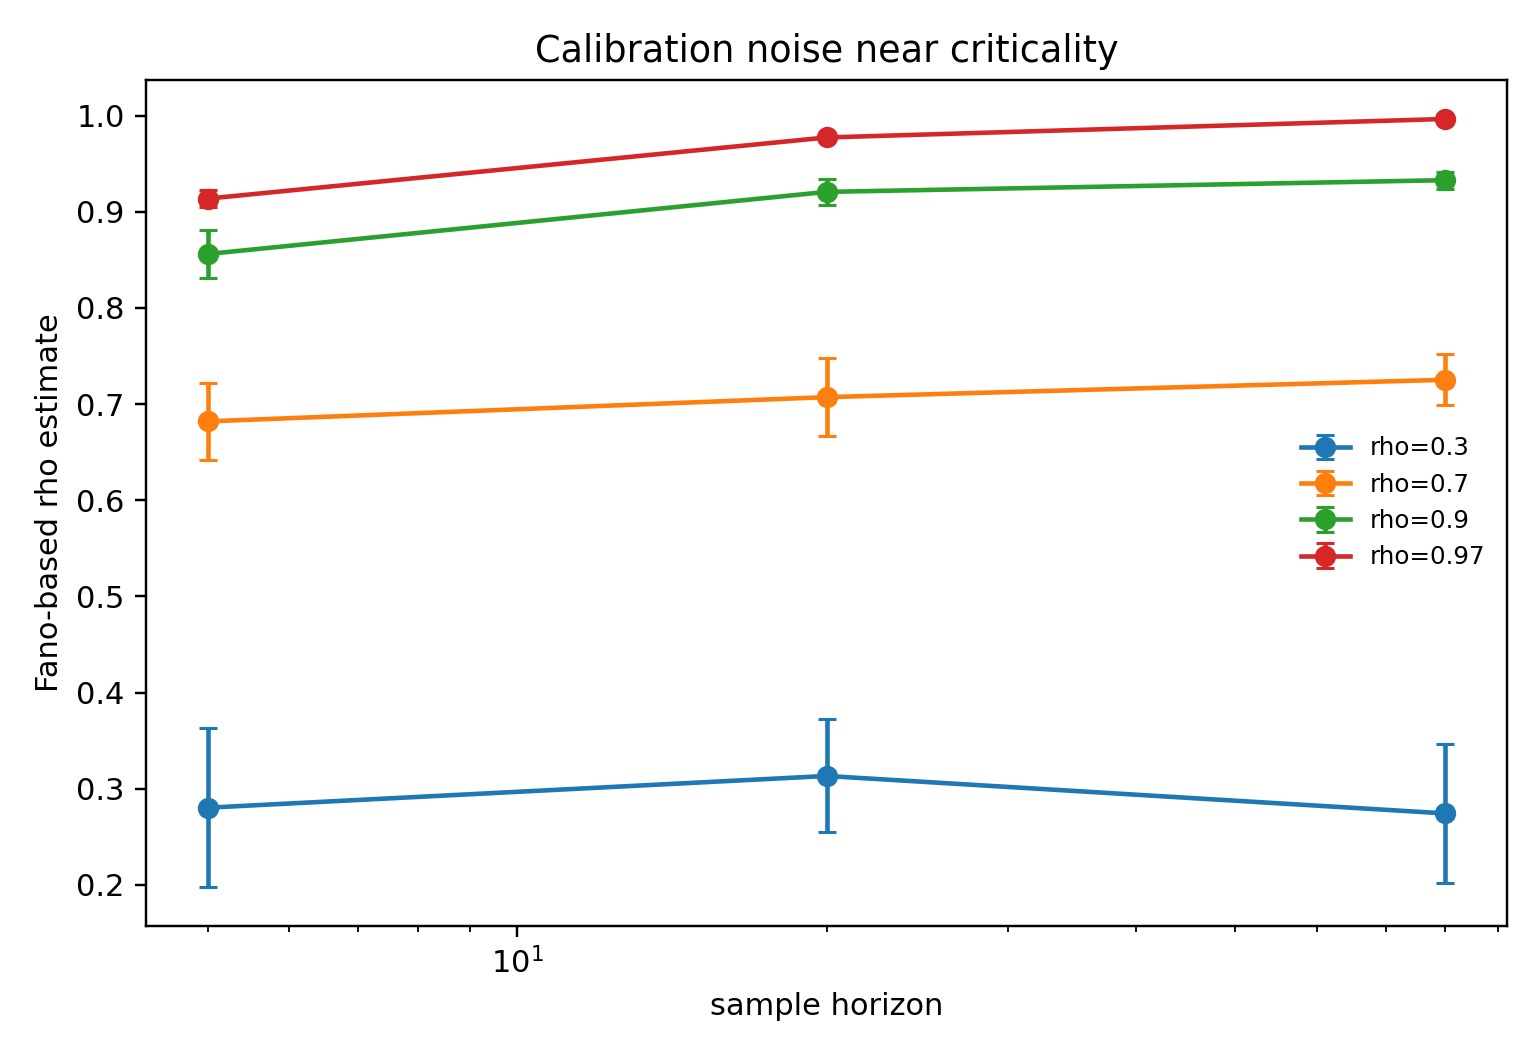
\includegraphics[width=.72\linewidth]{../results/figures/calibration_noise.png}
\caption{Fano-based criticality estimates across horizons.}
\end{figure}

\subsection{Robust DP}

The finite-scenario DP now includes explicit bid-side and ask-side no-quote
actions. In the full refreshed run, the raw DP action grid contains 9,947
two-sided quote states, 4,241 bid-only states, 4,241 ask-only states, and 579
full no-quote states. The first-step, zero-inventory policy switches to full
no-quote for $\hat\rho\ge0.97$ across the tested ambiguity radii. Averaged over
the DP grid, no-quote rates are $45.7\%$ under relative-slack ambiguity and
$49.6\%$ under absolute-Gamma ambiguity; full two-sided withdrawal rates are
$2.9\%$ and $3.2\%$, respectively. This is still a reduced Bellman
approximation, not a queue-calibrated quote-refusal simulator comparable
one-for-one with \cite{WangNoQuote2025}.

\begin{figure}[htbp]
\centering
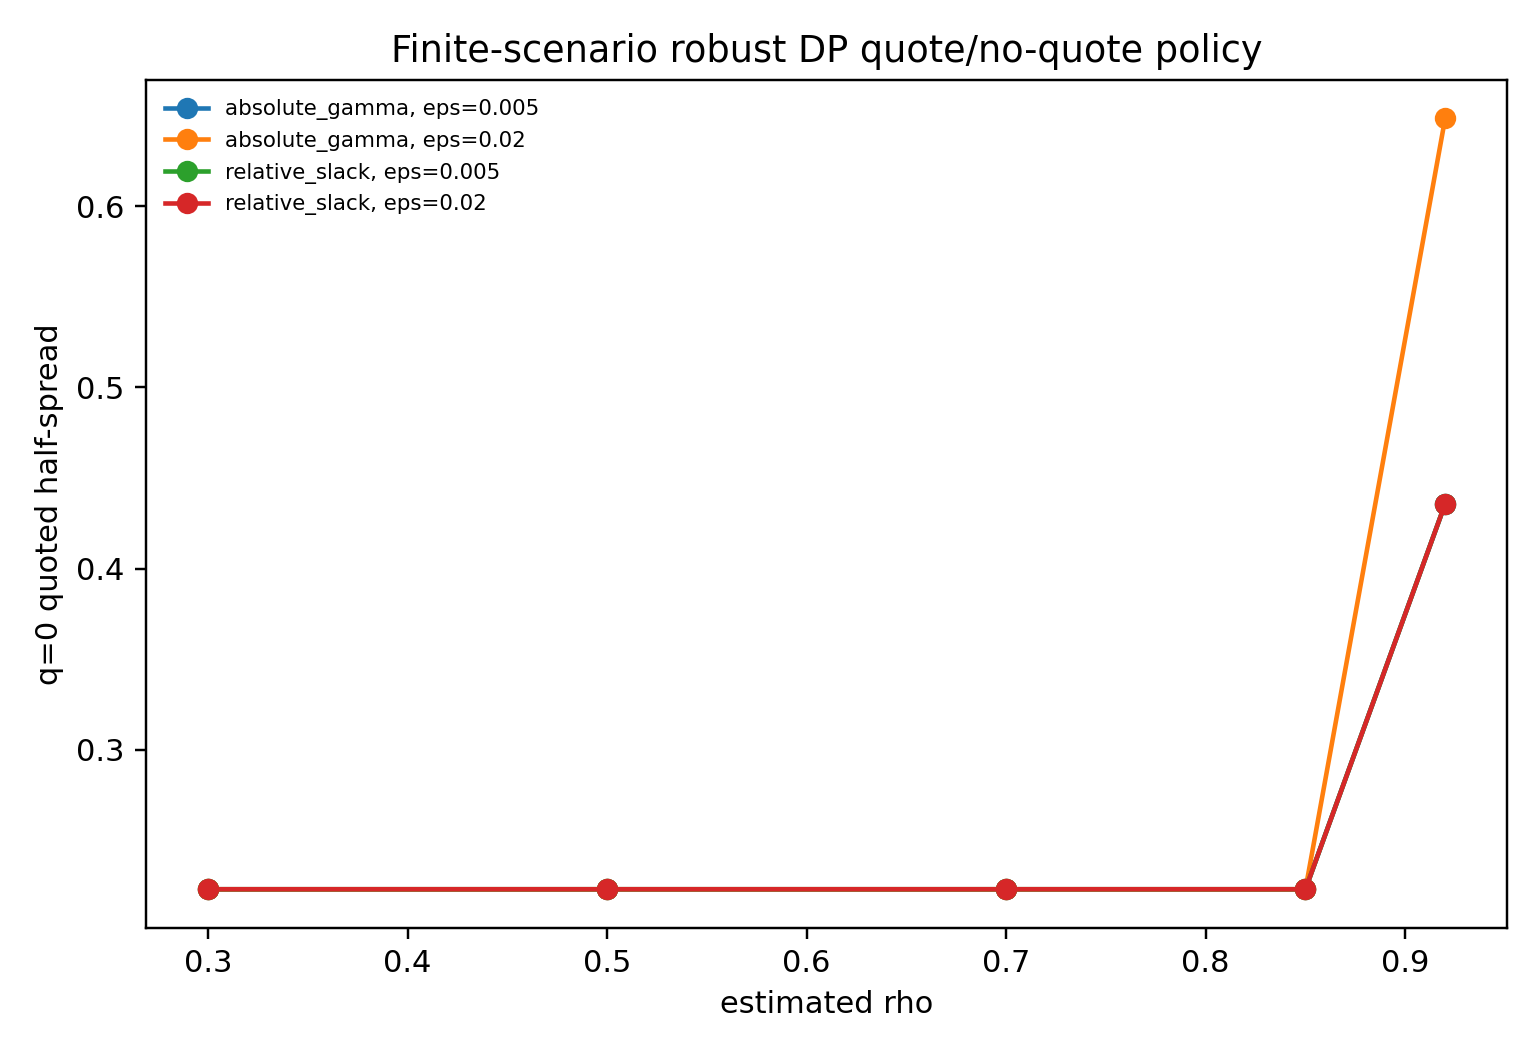
\includegraphics[width=.72\linewidth]{../results/figures/robust_dp_quotes.png}
\caption{Reduced robust-DP quoted half-spread and no-quote switching as
criticality increases.}
\end{figure}

To connect the local optimizer theorem to the implementation, we also run a
quote-map sensitivity diagnostic. For the smooth implemented half-spread,
nominal and relative-Gamma robust policies recover critical exponent $3.000$
for $d\delta/d\rho$, while absolute-Gamma robust policies approach exponent
$4.000$ in the uncapped interior region. Capped or no-quote points are marked
as nonsmooth active-set cases rather than treated as classical derivatives.

\begin{figure}[htbp]
\centering
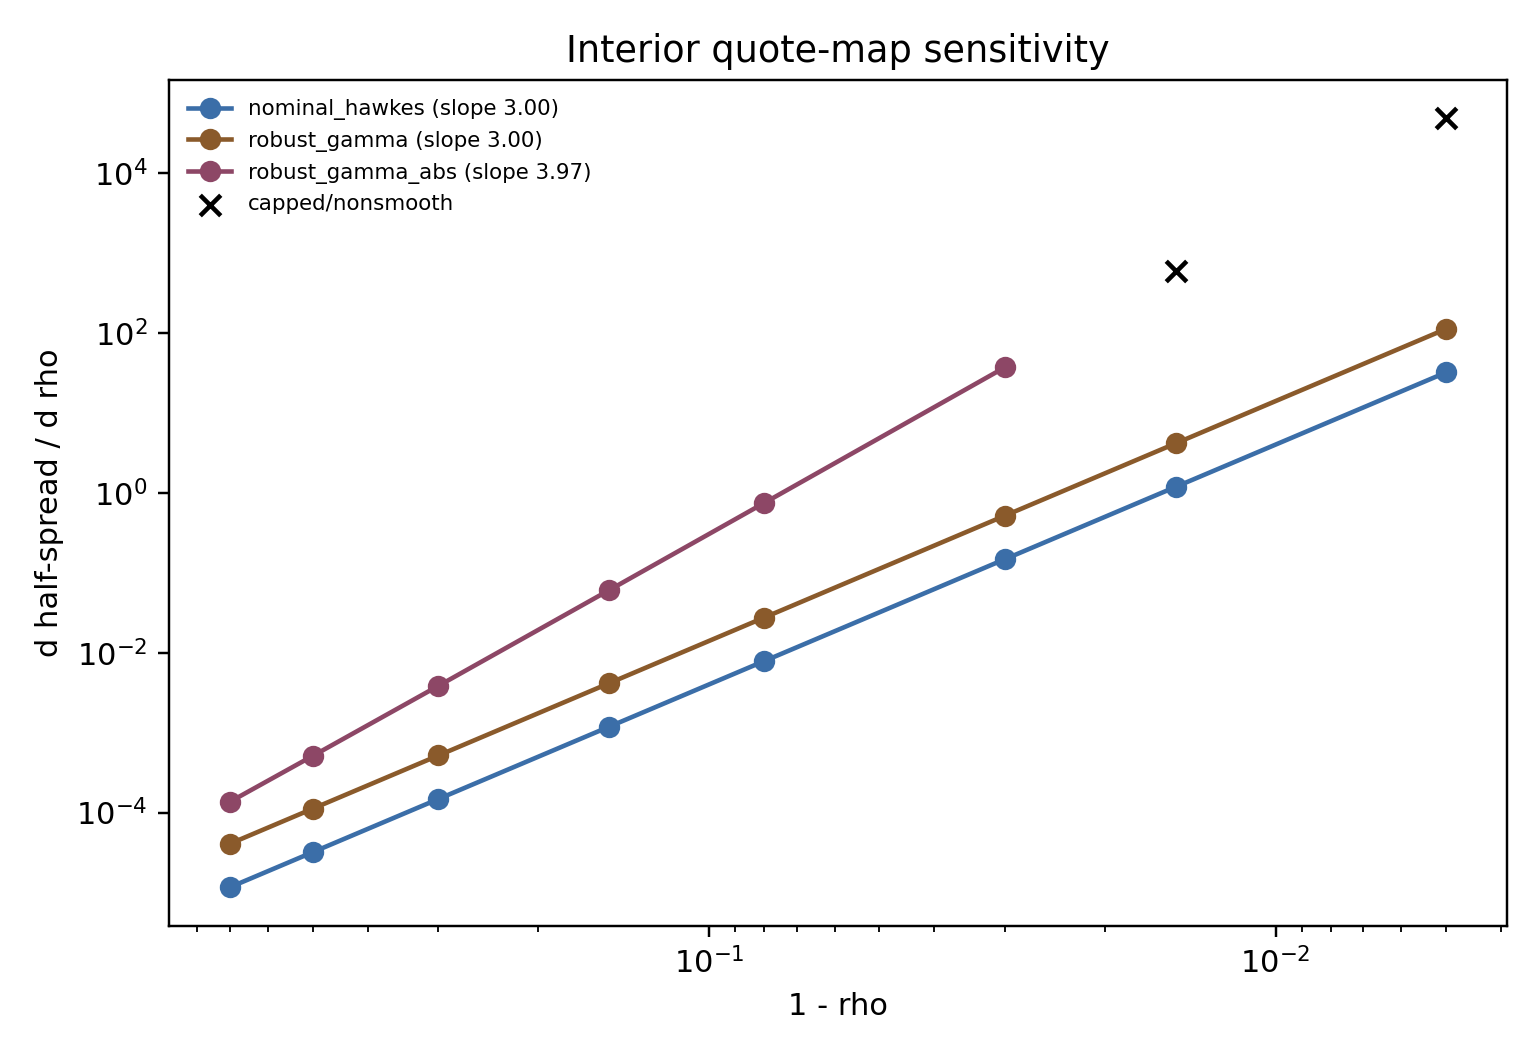
\includegraphics[width=.72\linewidth]{../results/figures/quote_sensitivity_diagnostic.png}
\caption{Interior quote-map sensitivity. Smooth relative-Gamma policies have
third-order derivative blowup, while absolute-Gamma ambiguity has one
additional critical derivative factor until spread caps bind.}
\end{figure}

\subsection{Public Data Panels}

The public datasets are not used to prove the structural ambiguity theorem,
because the true $\Gamma$ is unobserved. They establish empirical plausibility
for clustered order flow and overdispersed liquidity states. Binance aggregate
trades are fetched from the public archive at
\url{https://data.binance.vision/data/spot/daily/aggTrades/}.

\begin{table}[htbp]
\centering
\small
\begin{tabular}{@{}lrrrr@{}}
\toprule
Ticker & Rows & Events/sec & Event Fano & Mean spread \\
\midrule
AAPL & 118497 & 5.064 & 19.460 & 0.155 \\
AMZN & 57515 & 2.458 & 13.329 & 0.136 \\
GOOG & 49482 & 2.115 & 17.185 & 0.311 \\
INTC & 404986 & 17.307 & 220.650 & 0.013 \\
MSFT & 411409 & 17.582 & 196.485 & 0.013 \\
\bottomrule
\end{tabular}
\caption{Public LOBSTER sample sanity panel.}
\end{table}

\begin{table}[htbp]
\centering
\small
\begin{tabular}{@{}lrrrr@{}}
\toprule
Symbol & Agg. trades & Agg. trades/sec & Event Fano & ACF1 \\
\midrule
BTCUSDT & 1364603 & 15.794 & 200.274 & 0.342 \\
ETHUSDT & 597417 & 6.915 & 29.730 & 0.241 \\
SOLUSDT & 218278 & 2.526 & 12.240 & 0.201 \\
\bottomrule
\end{tabular}
\caption{Public Binance aggregate-trade event panel for 2024-01-15.}
\end{table}

\begin{table}[htbp]
\centering
\small
\begin{tabular}{@{}lrrrr@{}}
\toprule
Symbol & Rows & Rel. spread bps & Return std & Depth Fano \\
\midrule
BTC & 10081 & 0.163 & 0.000687 & 33.989 \\
ETH & 10081 & 0.591 & 0.000910 & 513.703 \\
SOL & 10080 & 0.911 & 0.001110 & 1697.605 \\
\bottomrule
\end{tabular}
\caption{Public crypto L2 depth sanity panel.}
\end{table}

\begin{figure}[htbp]
\centering
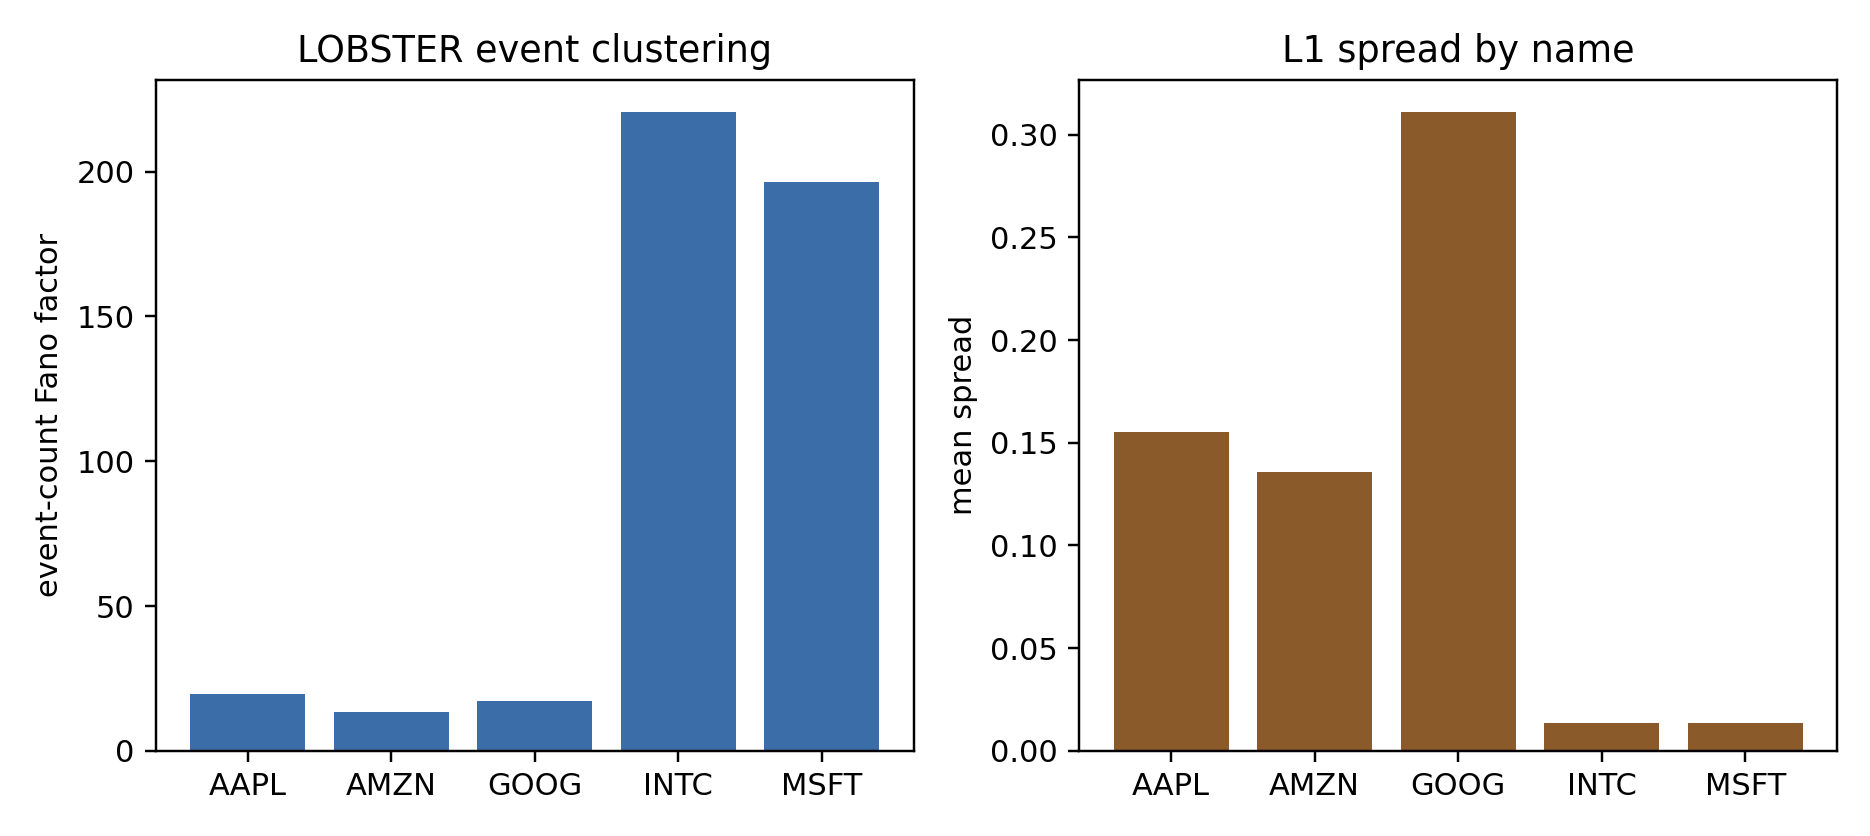
\includegraphics[width=.49\linewidth]{../results/figures/lobster_panel_sanity.png}
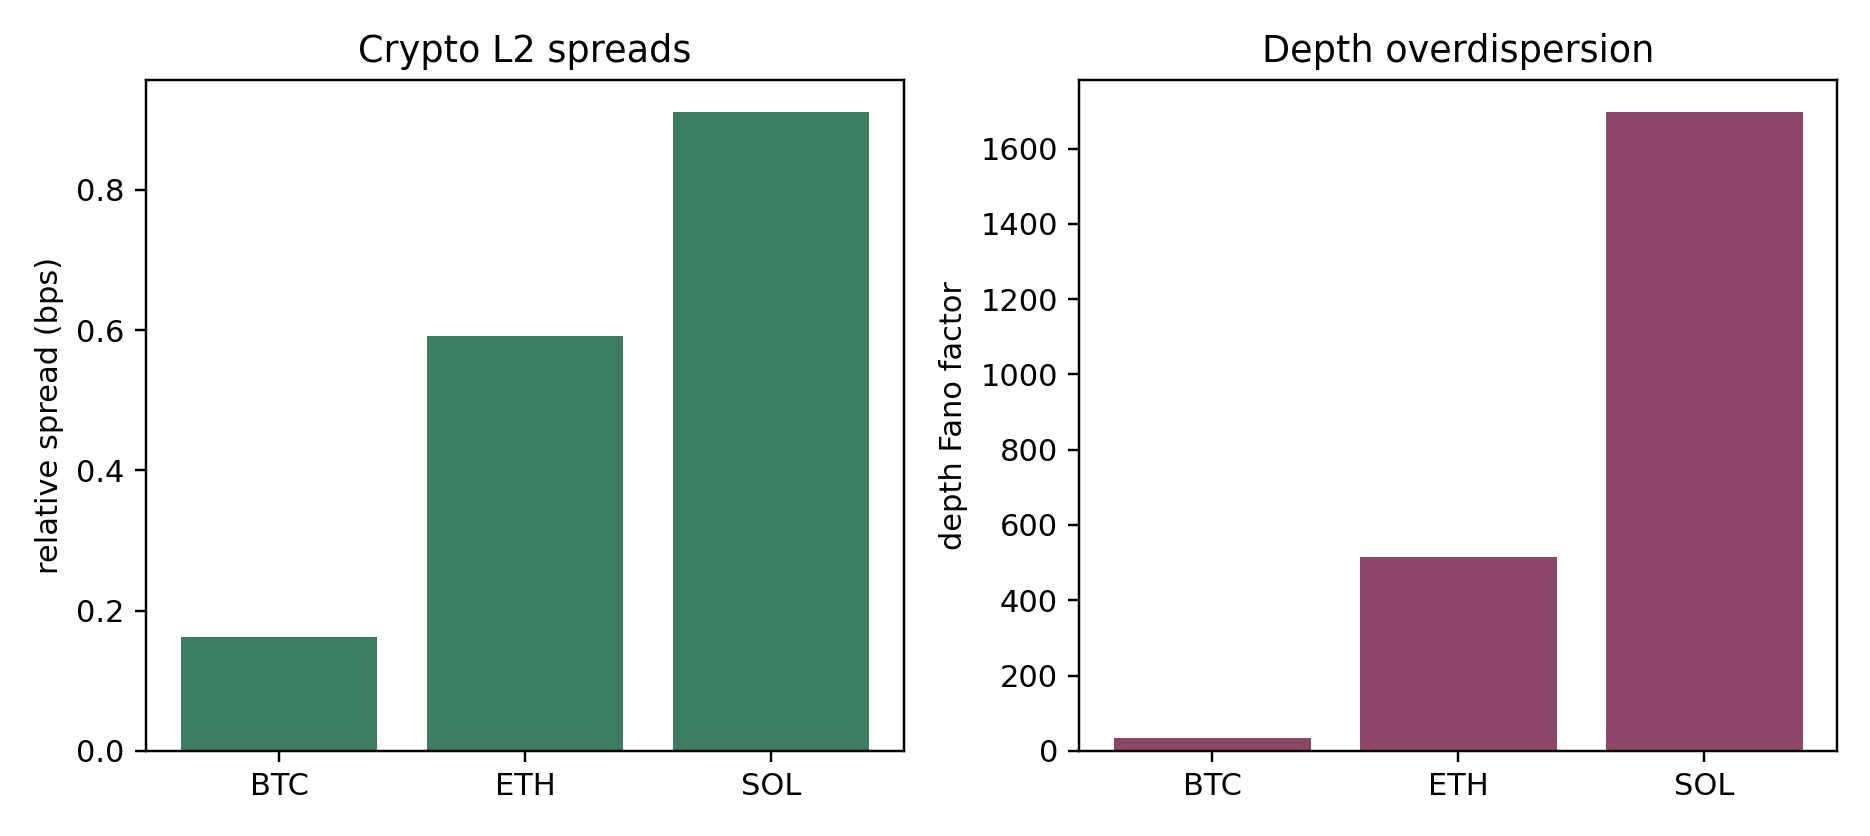
\includegraphics[width=.49\linewidth]{../results/figures/crypto_l2_sanity.png}
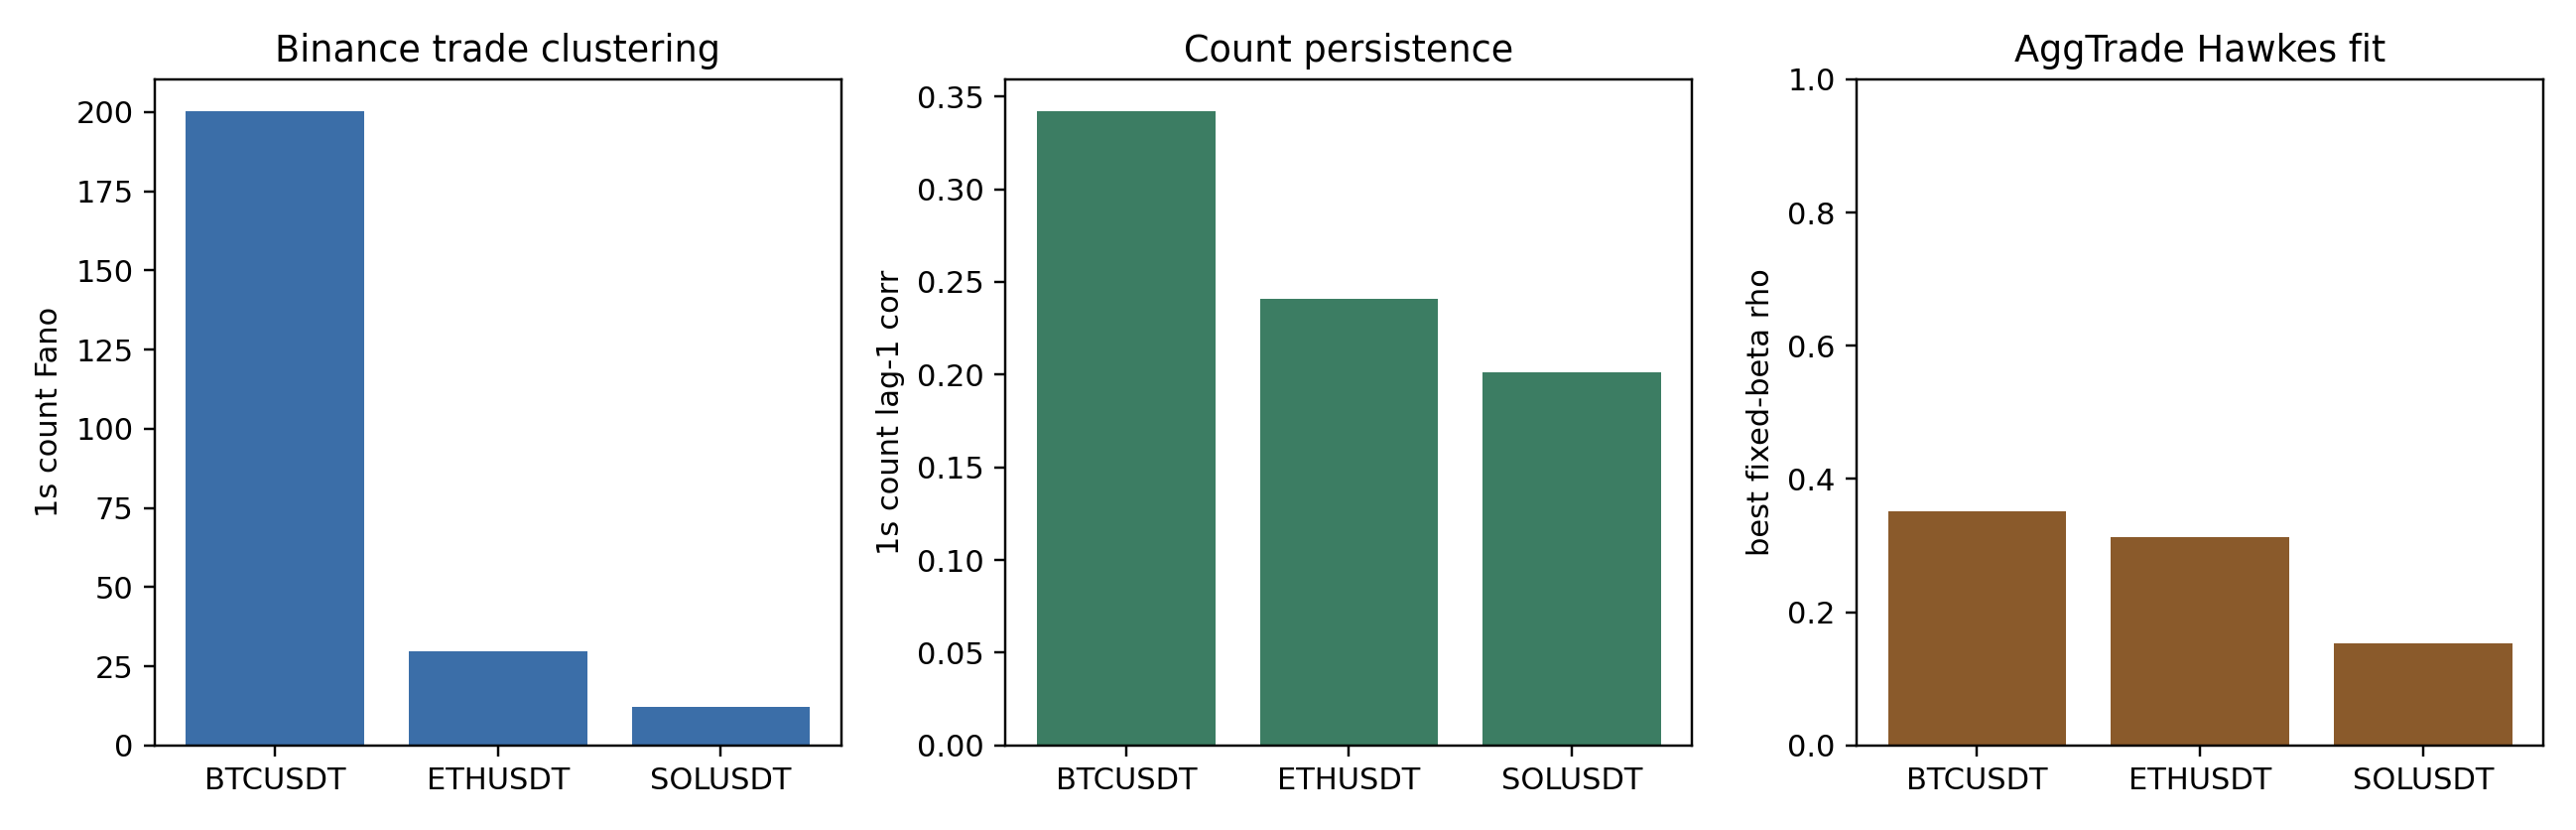
\includegraphics[width=.78\linewidth]{../results/figures/binance_aggtrades_hawkes.png}
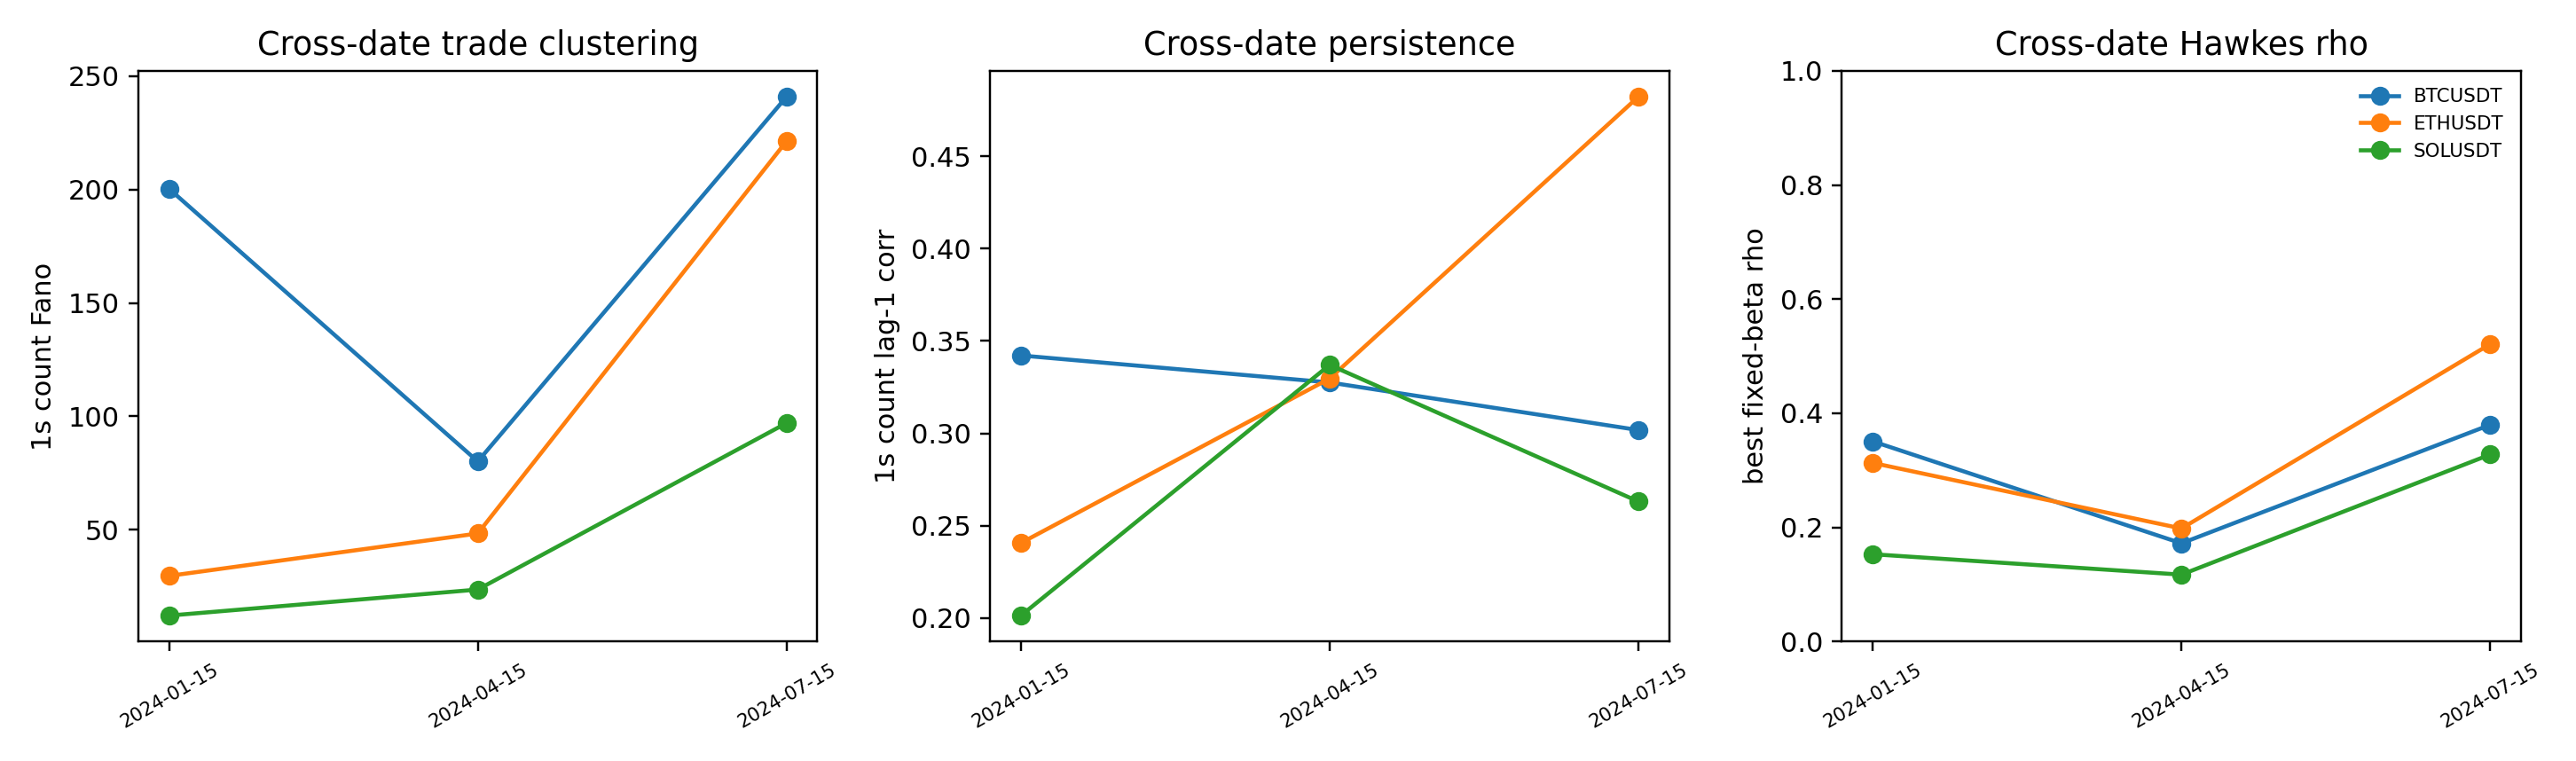
\includegraphics[width=.86\linewidth]{../results/figures/binance_aggtrades_cross_date_hawkes.png}
\caption{Public-data sanity figures: LOBSTER event clustering and spreads,
crypto L2 spreads and depth overdispersion, Binance aggregate-trade clustering,
fixed-beta Hawkes diagnostics, and cross-date robustness.}
\end{figure}

\subsection{Corrected Hawkes Calibration Diagnostics}

Before interpreting real-data Hawkes fits, we validated the corrected
single-exponential MLE on Ogata-simulated paths with known parameters. The
validation recovers moderate and near-critical branching ratios without
beta-bound failures.

\begin{table}[htbp]
\centering
\small
\begin{tabular}{@{}rrrrr@{}}
\toprule
$\rho$ true & $\beta$ true & $\rho$ MAE & $\beta$ MAPE & Beta cap rate \\
\midrule
0.30 & 2.0 & 0.043 & 0.201 & 0.000 \\
0.70 & 4.0 & 0.019 & 0.026 & 0.000 \\
0.90 & 8.0 & 0.016 & 0.039 & 0.000 \\
\bottomrule
\end{tabular}
\caption{Synthetic Ogata validation for the corrected Hawkes MLE.}
\end{table}

We additionally validate the fixed-beta marked multivariate estimator on
three-type Ogata Hawkes paths with known branching matrices. For target
spectral radii $0.35$ and $0.65$ at $\beta=3$, the marked estimator has
spectral-radius MAE $0.025$ and $0.023$, relative Frobenius branching-matrix
error $0.234$ and $0.133$, and success rate one. This check is important
because the public-data marked calibrations below are only meaningful if the
estimator recovers a known multitype $\Gamma$ under controlled simulation.

\begin{table}[htbp]
\centering
\small
\begin{tabular}{@{}rrrrr@{}}
\toprule
$\rho$ true & Mean events & $\rho$ MAE & $\|\hat\Gamma-\Gamma\|_F/\|\Gamma\|_F$ & Success \\
\midrule
0.35 & 1209.8 & 0.025 & 0.234 & 1.000 \\
0.65 & 2171.2 & 0.023 & 0.133 & 1.000 \\
\bottomrule
\end{tabular}
\caption{Synthetic Ogata validation for the fixed-beta marked multivariate
Hawkes estimator.}
\end{table}

\begin{figure}[htbp]
\centering
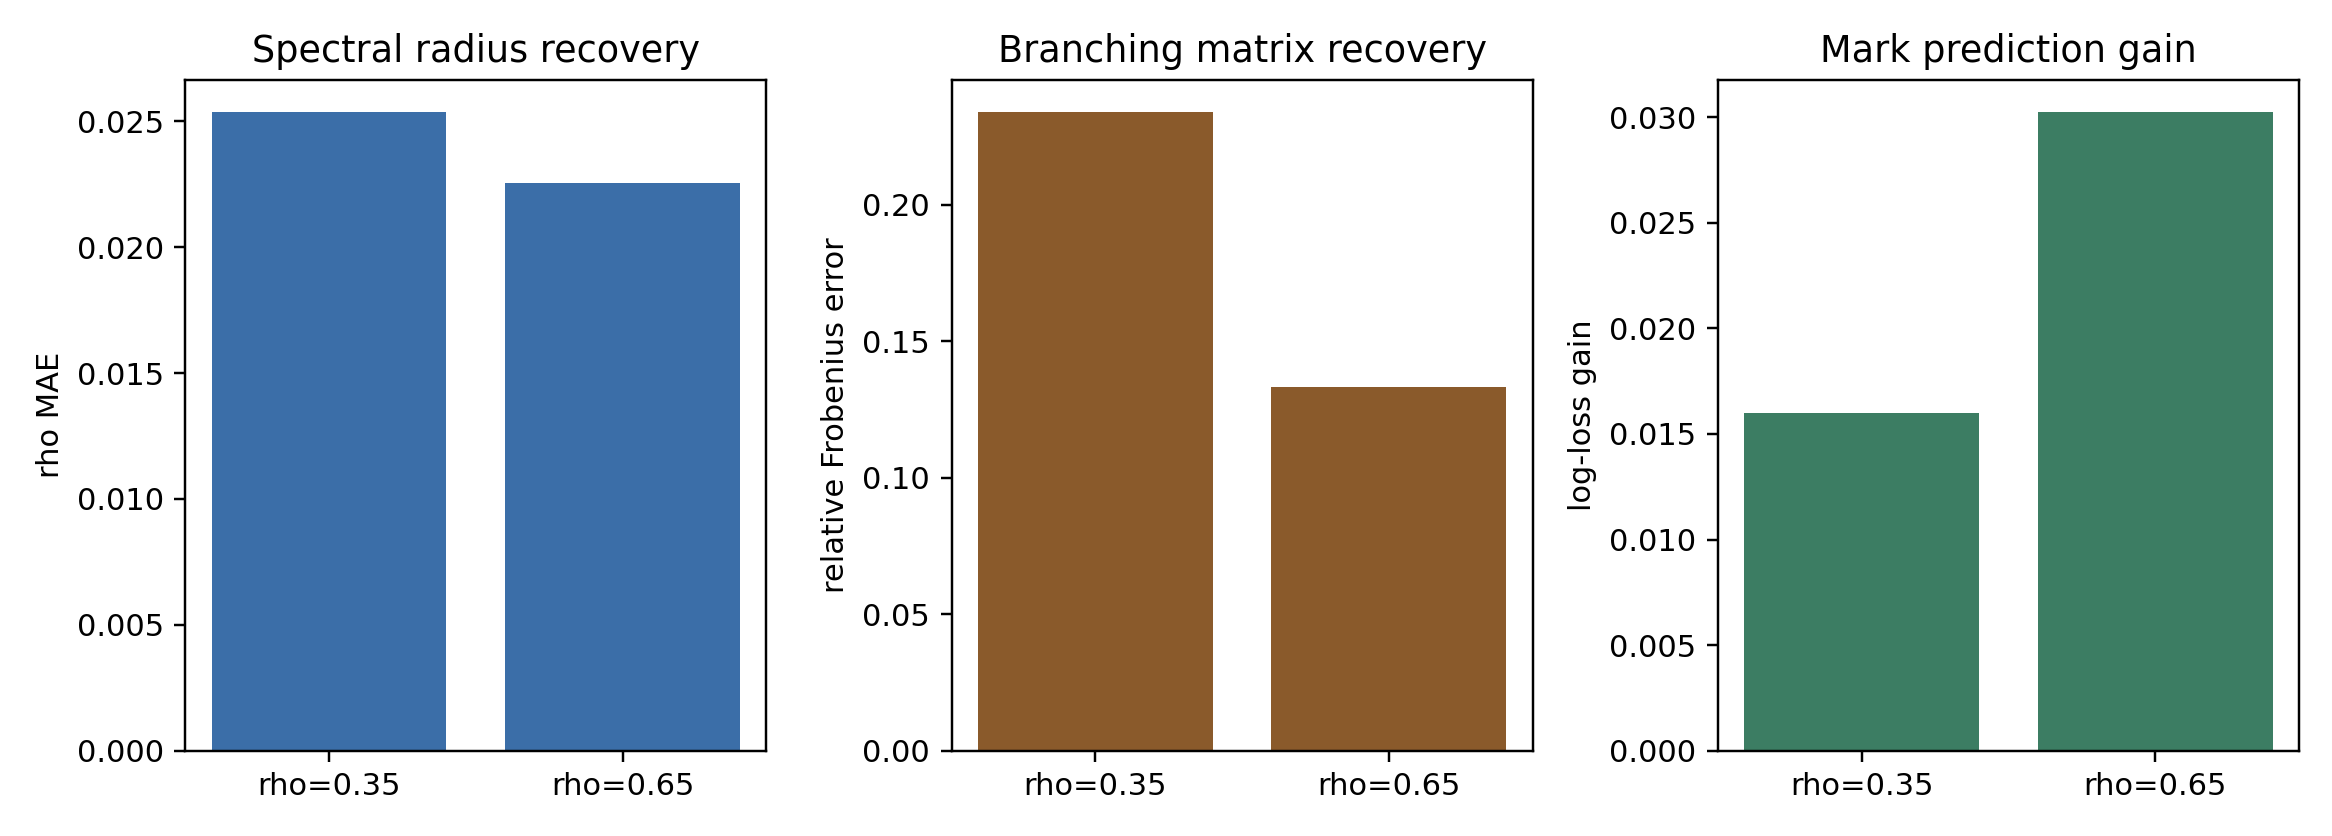
\includegraphics[width=.76\linewidth]{../results/figures/lobster_marked_hawkes_estimator_validation.png}
\caption{Marked multivariate Ogata validation: spectral-radius recovery,
branching-matrix recovery, and conditional mark-prediction gain.}
\end{figure}

The Binance aggregate-trade panel provides a separate public crypto event
check. On 2024-01-15, BTCUSDT, ETHUSDT, and SOLUSDT have 218k to 1.36m
aggregate trades, one-second event-count Fano factors from $12.24$ to
$200.27$, and lag-one count autocorrelations from $0.201$ to $0.342$. Fixed
beta Hawkes fits over all aggregate trades, buy-aggressor trades, and
sell-aggressor trades select $\beta=100$ in the current grid. All-trade
branching ratios are $0.351$ for BTCUSDT, $0.313$ for ETHUSDT, and $0.153$ for
SOLUSDT; sell-aggressor branching is higher for BTCUSDT and ETHUSDT, at
$0.493$ and $0.463$. This is useful cross-asset evidence of clustered event
flow, but aggregate trades do not include order placement, cancellation, or
queue state, so the panel is not an execution benchmark.

To avoid relying on one crypto day, we repeat the Binance check on
2024-01-15, 2024-04-15, and 2024-07-15. Across all-event fixed-beta fits,
branching-ratio ranges are $0.172$--$0.380$ for BTCUSDT, $0.198$--$0.521$ for
ETHUSDT, and $0.117$--$0.328$ for SOLUSDT. The median all-event branching
ratios remain $0.351$, $0.313$, and $0.153$, respectively.

On raw LOBSTER message arrivals, however, the all-message single-exponential
fit remains a misspecification diagnostic rather than a structural calibration
target. The corrected all-message panel still places $\beta$ at the upper
bound for every ticker under the 100k-event cap, with fitted branching ratios
between $0.64$ and $0.76$. Event-type splits and fixed-beta profiles show that
branching estimates are sensitive to the assumed decay scale; timestamp
aggregation sharply reduces the fitted decay, with median $\beta$ falling from
$148.4$ on raw events to $23.4$ at 1ms aggregation and $1.46$ at 10ms
aggregation. A fixed-beta two-scale diagnostic improves the empirical picture
but does not remove the misspecification warning: among the tested pairs, every
ticker/event-group selects $(\beta_{\rm slow},\beta_{\rm fast})=(1,100)$, and
median fast-excitation shares are $0.764$ for all messages, $0.723$ for limits,
$0.660$ for cancel/delete events, and $0.871$ for executions. Execution events
remain the hardest to fit, with median residual KS statistic about $0.415$.
This supports the methodological claim that raw unmarked message flows mix
multiple clocks and packet-level bursts, so robust market-making experiments
should use marked or multiscale calibration diagnostics, or report residual diagnostics
\cite{BacryMuzy2015,Ogata1988}.

The current package therefore adds a grouped marked multivariate Hawkes fit on
limit, cancel/delete, and execution event groups. With fixed exponential decay,
AIC selects $\beta=100$ for all five public LOBSTER tickers. The estimated
branching matrices are stable, with spectral radii from $0.367$ to $0.622$,
and the conditional mark log-loss improves over unconditional event-frequency
prediction by $0.005$ to $0.114$ nats per event. The median branching matrix
has the strongest source column from execution events, with median total
outgoing branching about $0.923$, and the largest median target row into limit
intensity, about $0.897$. Residual KS statistics still range from $0.050$ to
$0.217$, so the fit should be read as a reproducible marked calibration
diagnostic, not as a production-grade structural $\Gamma$ estimate.

Finally, to align the empirical object with the bid/ask control model, we fit a
six-mark side-aware Hawkes model using LOBSTER direction labels: limit,
cancel/delete, and execution events on buy and sell sides. AIC again selects
$\beta=100$ for all five tickers. The full six-mark branching matrices remain
stable, with spectral radii from $0.369$ to $0.624$, while conditional
six-mark log-loss improves over unconditional mark frequencies by $0.101$ to
$0.292$ nats per event. Median side-aggregated branching is strongest within
side, about $1.354$ from buy to buy and $1.403$ from sell to sell, with smaller
cross-side totals of about $0.492$ from buy to sell and $0.414$ from sell to
buy. The aggregate row sums can exceed one because they sum many target/source
entries; stability is assessed by the spectral radius of the full six-mark
matrix.

We then condition the six-mark time-rescaling residuals on observable L1 state
variables: event group, side, within-ticker size bucket, spread bucket,
top-depth bucket, and order-book imbalance bucket. This is intentionally a
misspecification audit rather than another fitted model. Across the five
public LOBSTER samples, wide-spread states have median residual mean $0.886$
and median KS statistic $0.220$, while tight-spread states have median residual
mean $1.110$ and median KS statistic $0.092$. Large-size events have residual
mean $0.828$ versus $1.018$ for small events. Execution marks show the largest
conditional mark-prediction gain, with median log-loss improvement $0.384$
nats per event. The result sharpens the empirical conclusion: side-aware
excitation is informative, but the residuals still depend materially on size
and book state.

\begin{figure}[htbp]
\centering
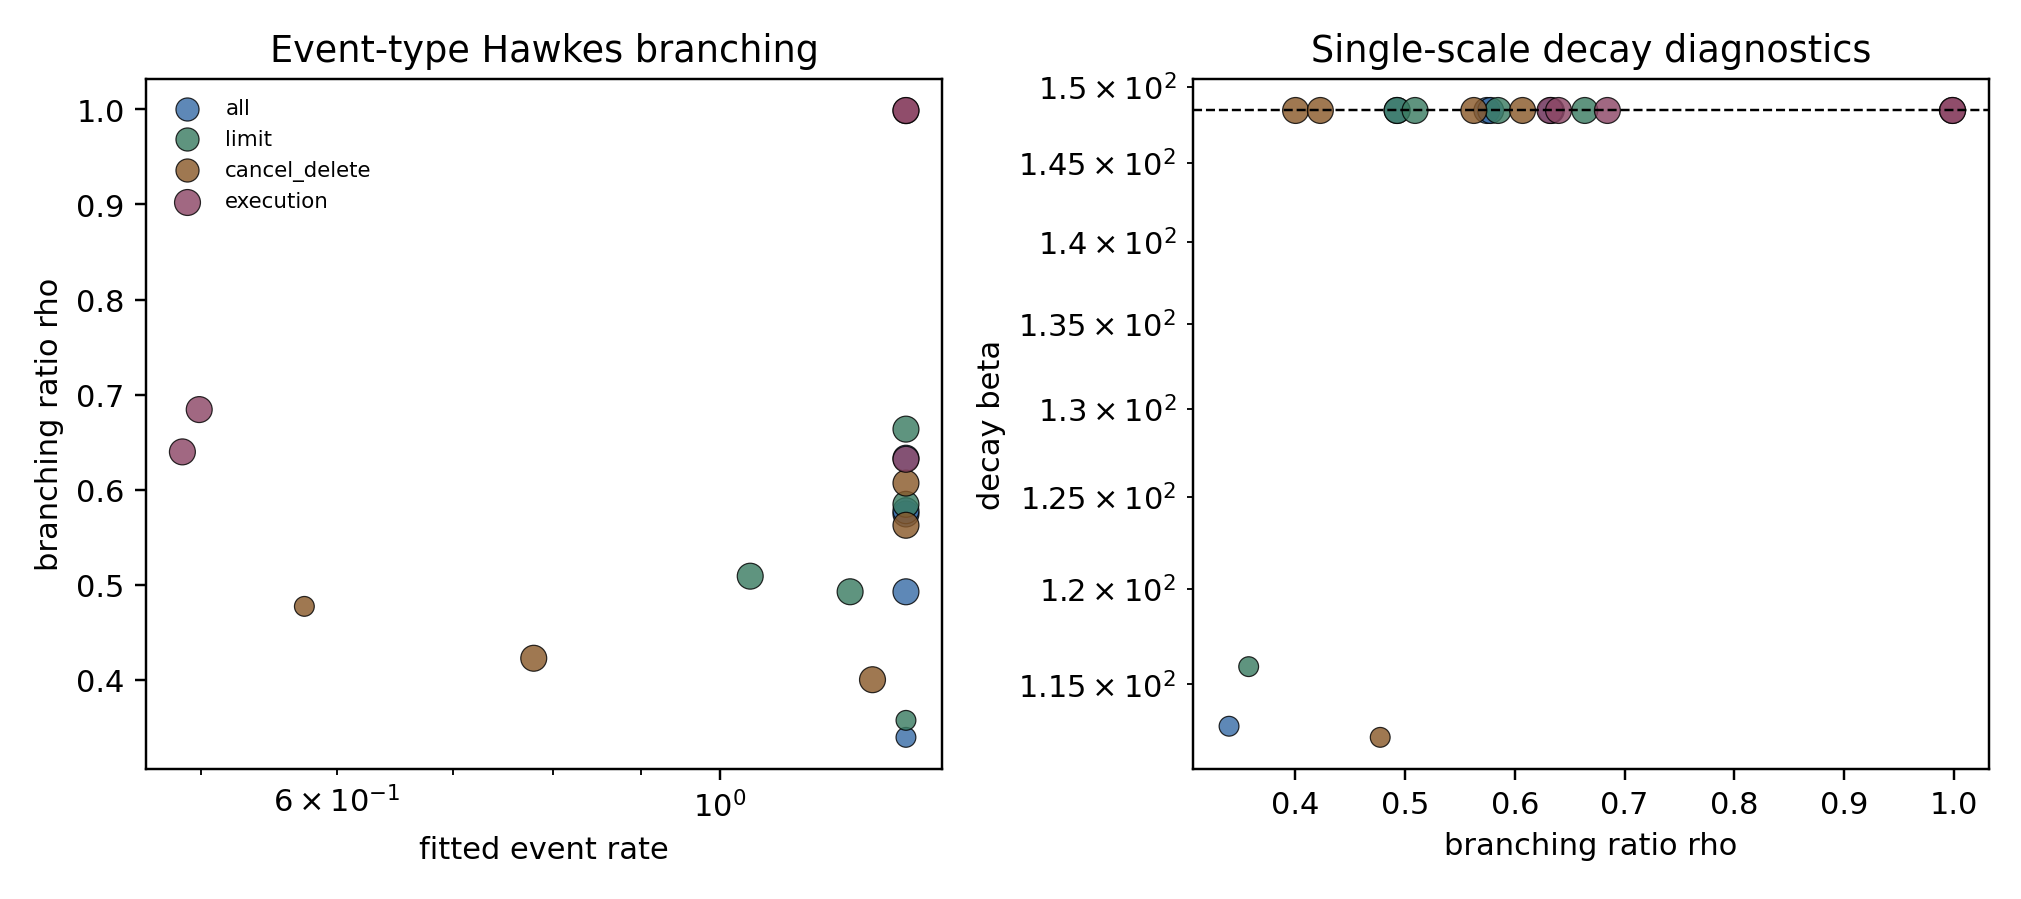
\includegraphics[width=.49\linewidth]{../results/figures/lobster_hawkes_event_type_rho_beta.png}
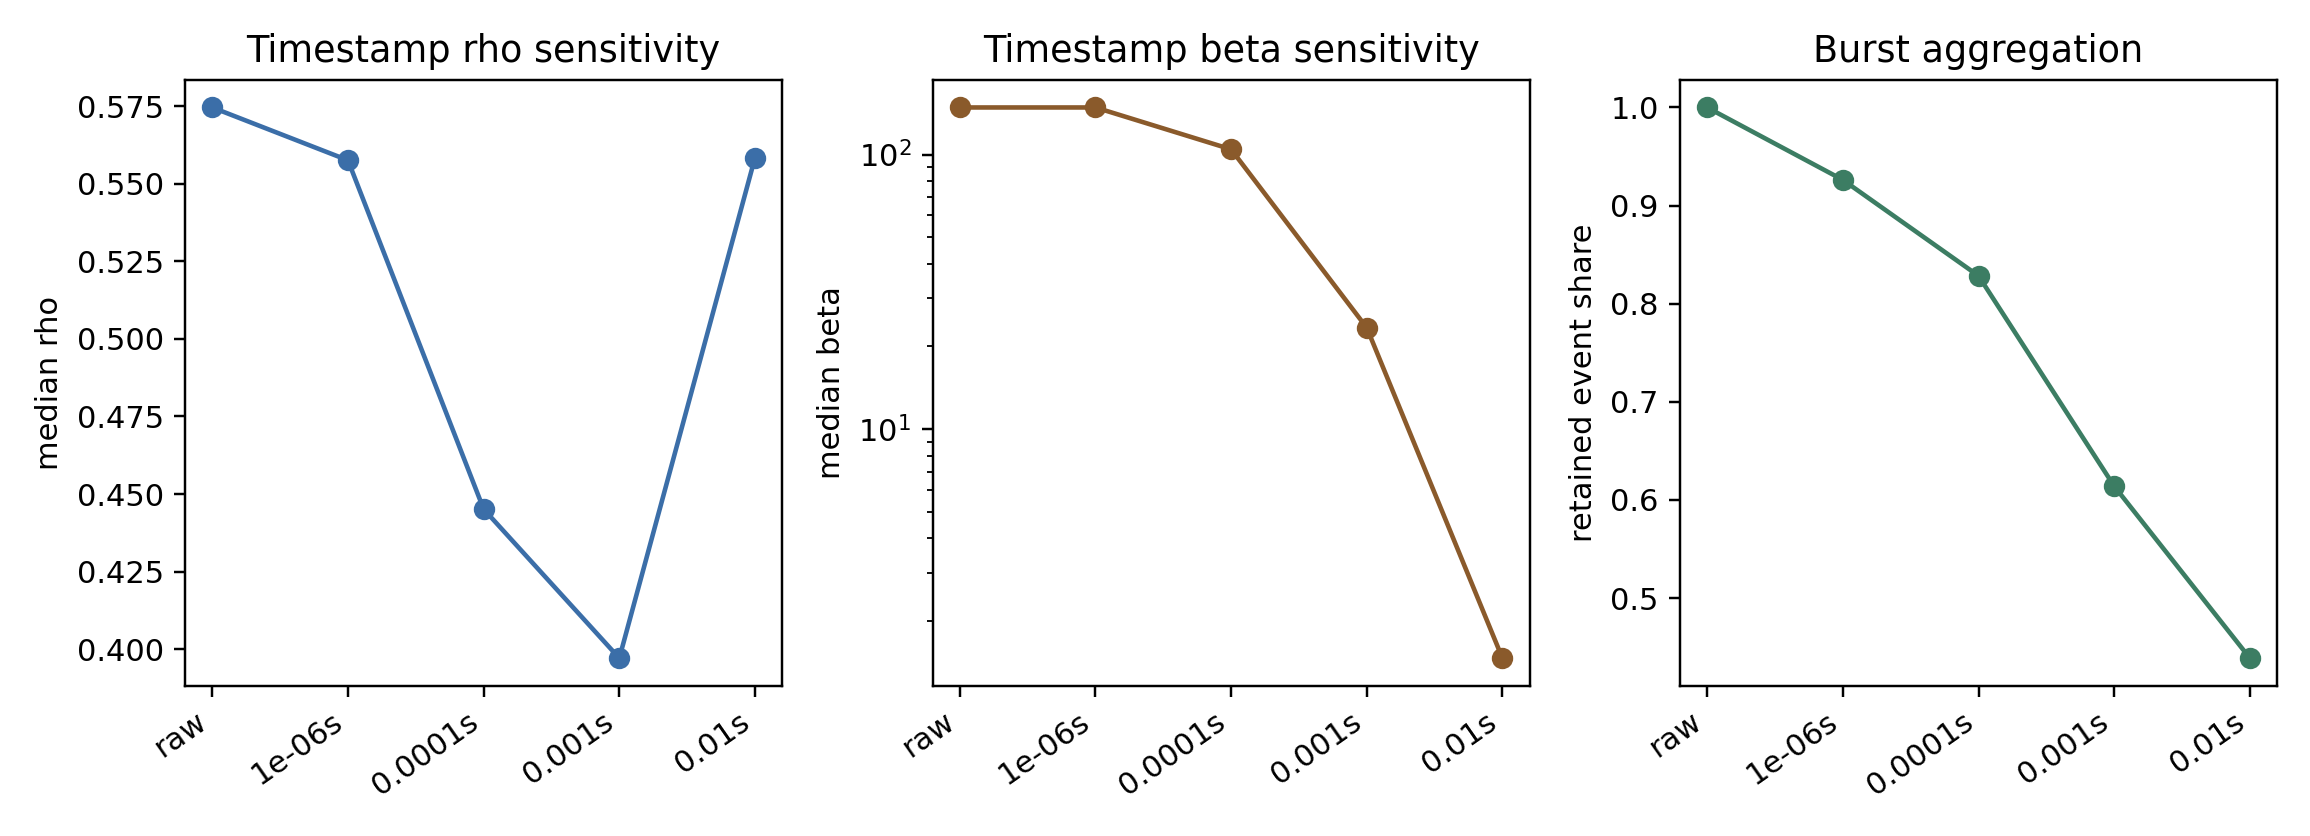
\includegraphics[width=.49\linewidth]{../results/figures/lobster_timestamp_resolution_sensitivity.png}
\caption{Corrected public-data Hawkes diagnostics: event-type branching/decay
and timestamp-resolution sensitivity.}
\end{figure}

\begin{figure}[htbp]
\centering
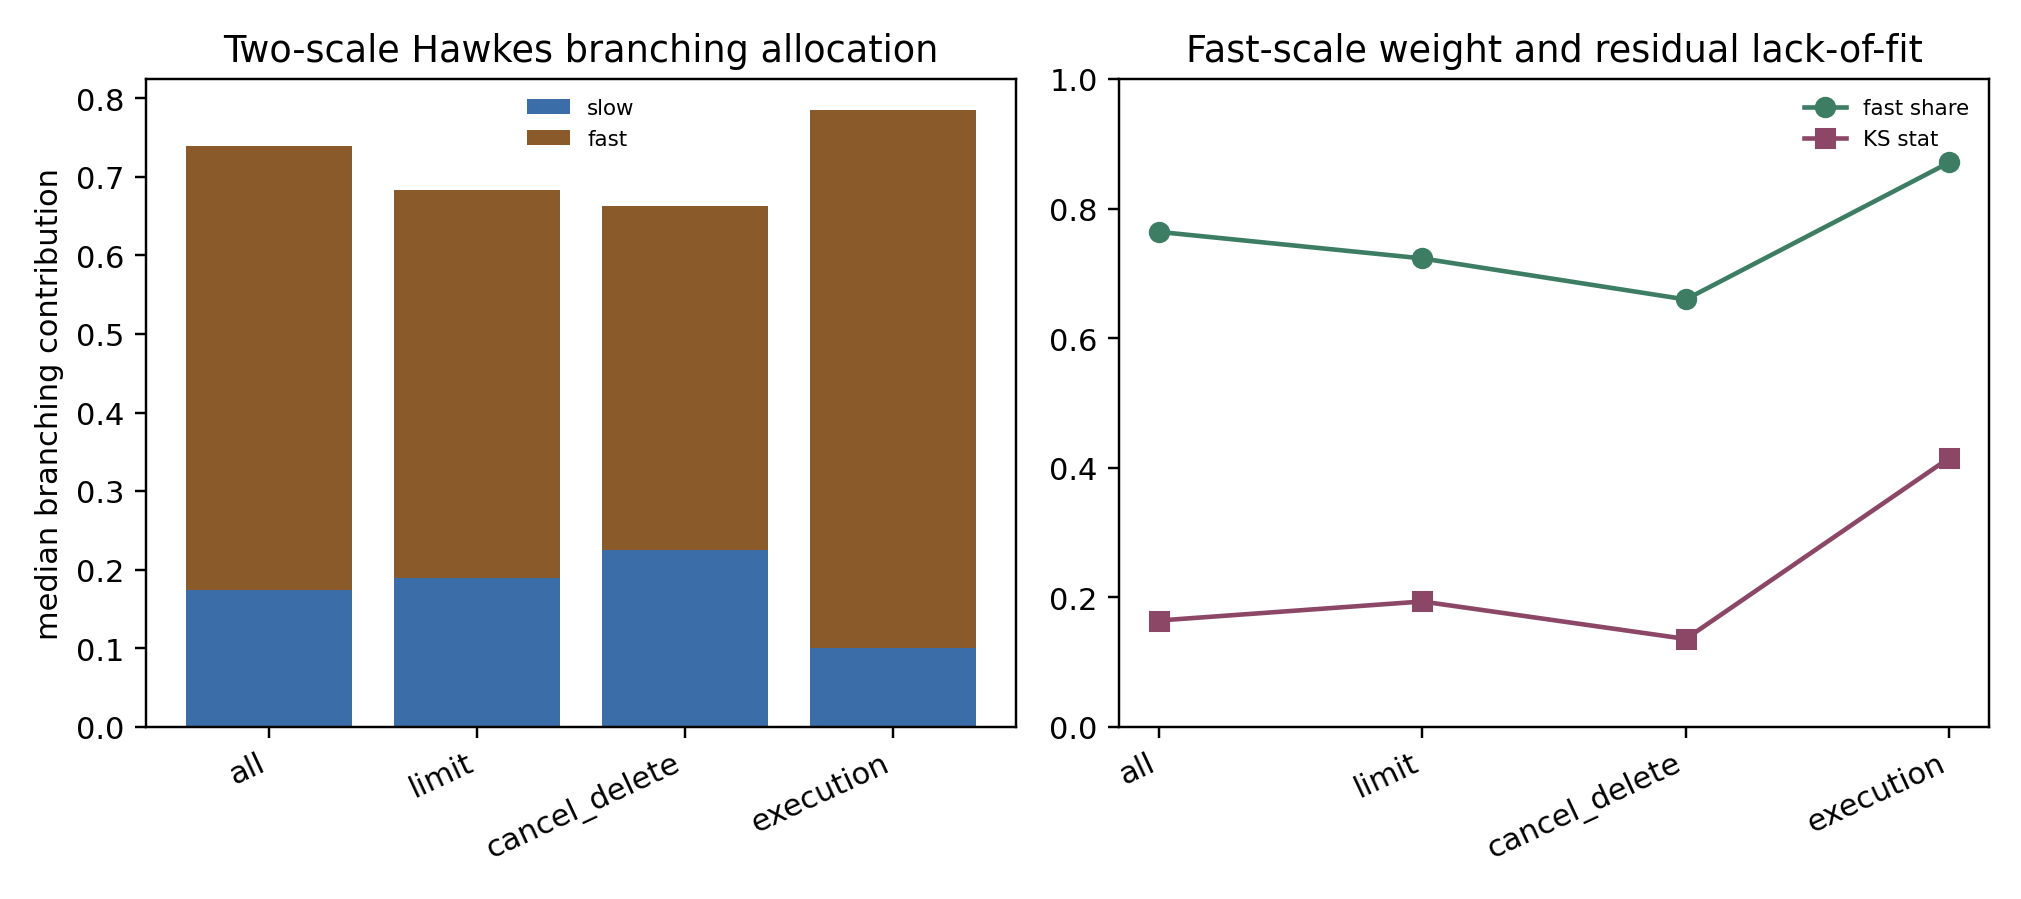
\includegraphics[width=.74\linewidth]{../results/figures/lobster_hawkes_multiscale.png}
\caption{Fixed-beta two-scale public-data Hawkes diagnostics. The selected
two-scale fits concentrate excitation on the fast component, especially for
execution events, while residual tests still flag misspecification.}
\end{figure}

\begin{figure}[htbp]
\centering
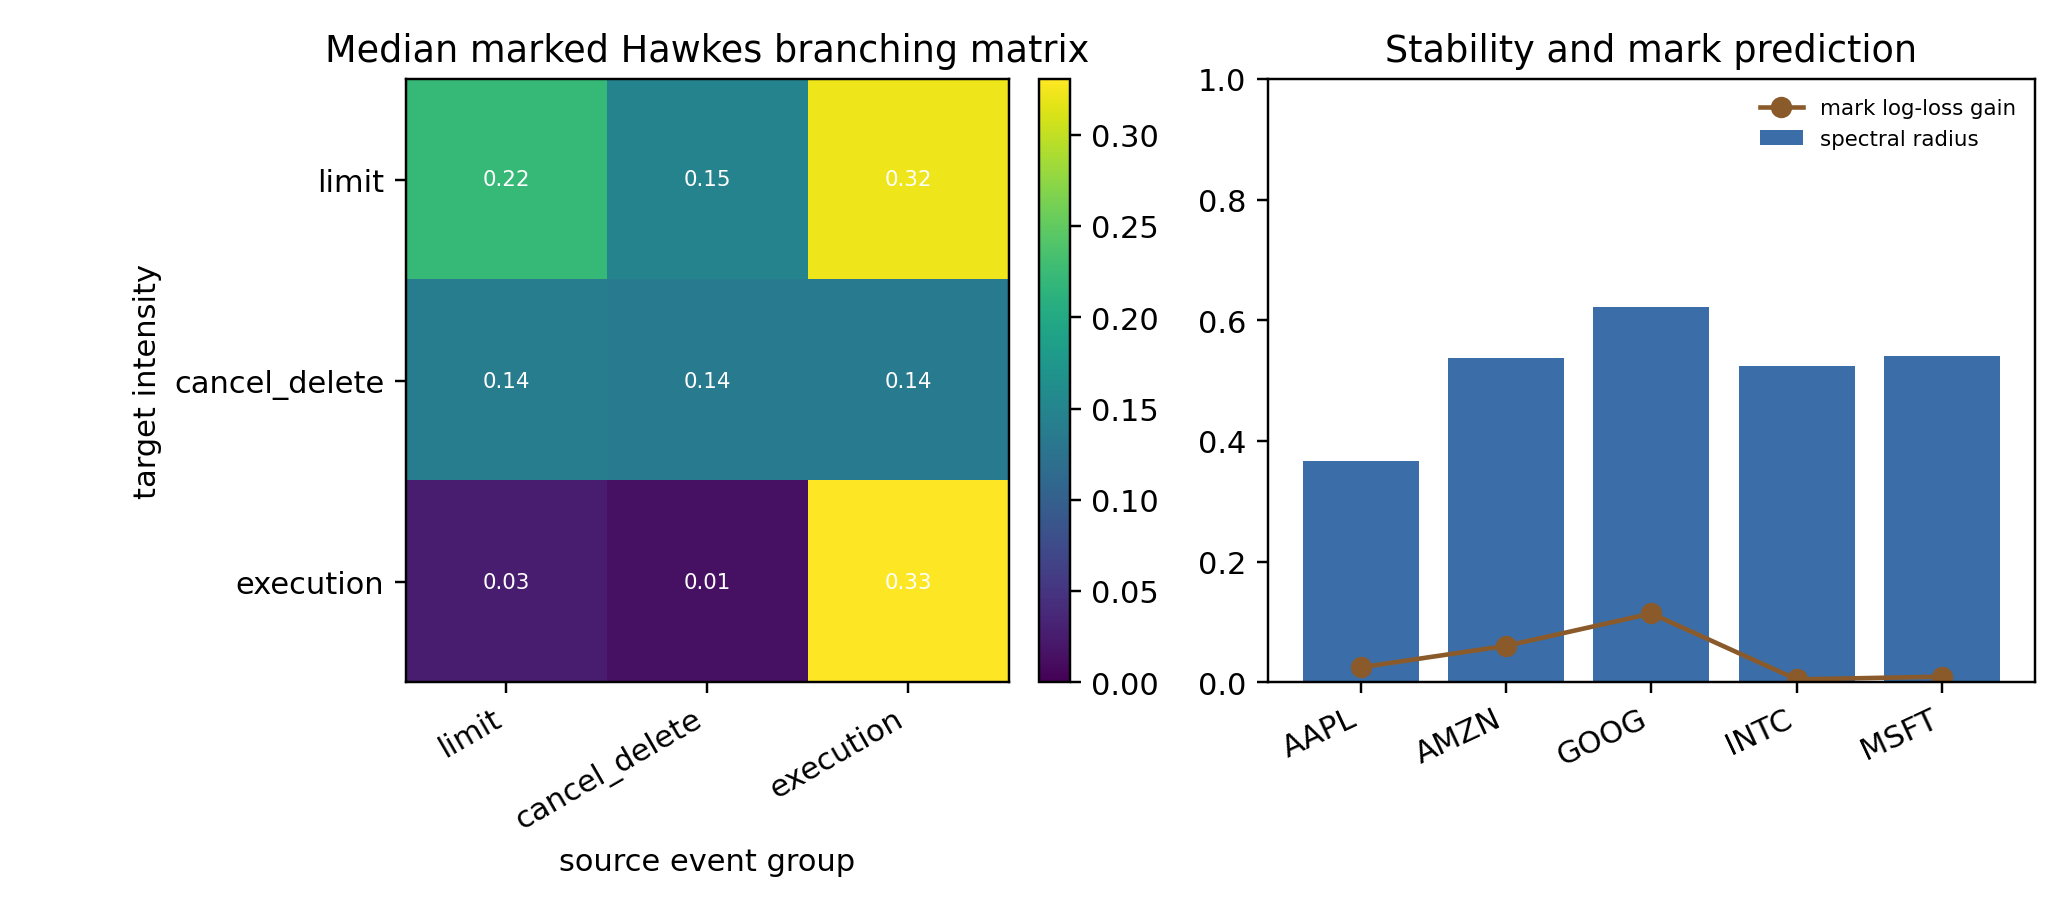
\includegraphics[width=.74\linewidth]{../results/figures/lobster_marked_hawkes_multivariate.png}
\caption{Grouped marked multivariate Hawkes diagnostics on LOBSTER limit,
cancel/delete, and execution events. The fixed-beta fits estimate stable
branching matrices and improve conditional mark prediction, but residual tests
still motivate richer side, size, and multiscale calibration.}
\end{figure}

\begin{figure}[htbp]
\centering
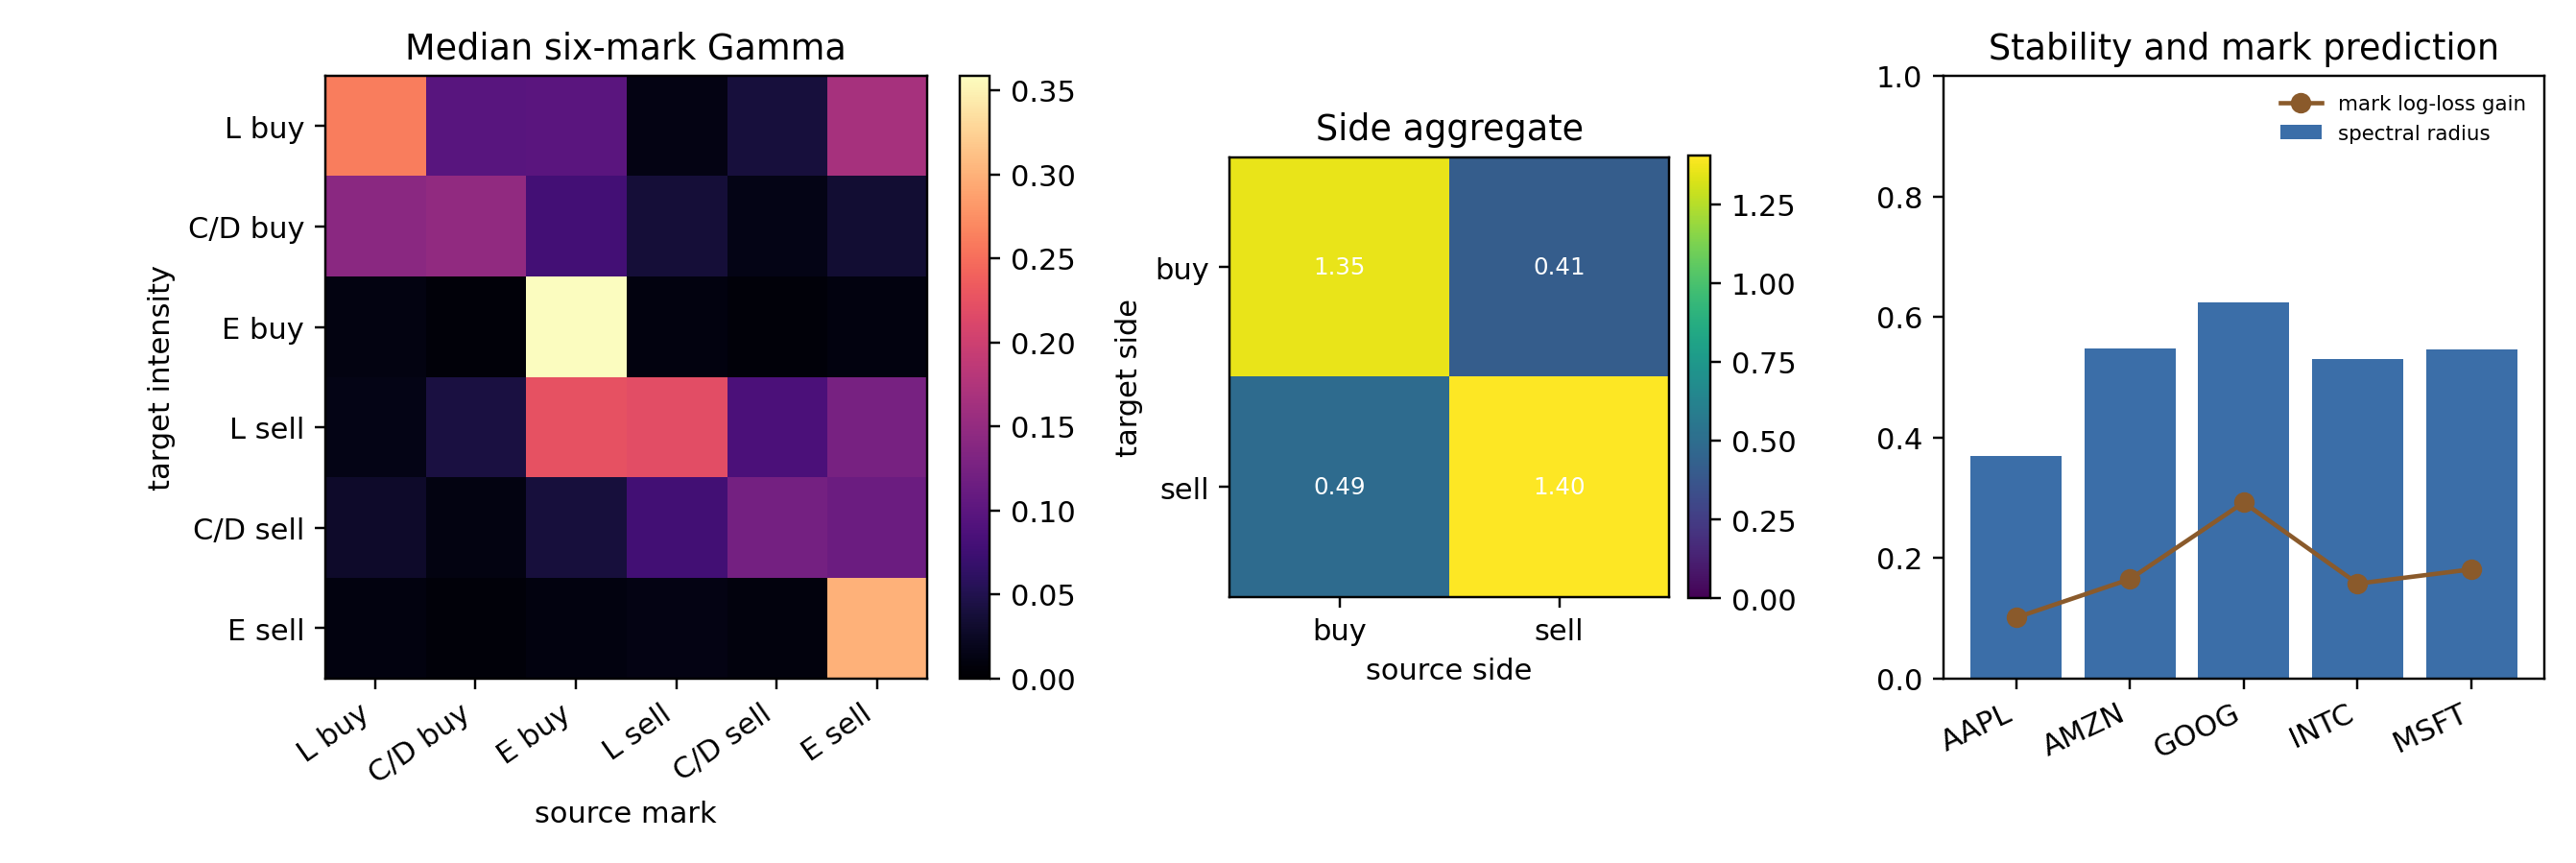
\includegraphics[width=.88\linewidth]{../results/figures/lobster_side_marked_hawkes_multivariate.png}
\caption{Side-aware marked multivariate Hawkes diagnostics using LOBSTER
direction labels. The six-mark fits bridge the empirical calibration object
toward bid/ask robust control, while remaining fixed-decay and message-side
rather than queue-position or size-aware.}
\end{figure}

\begin{figure}[htbp]
\centering
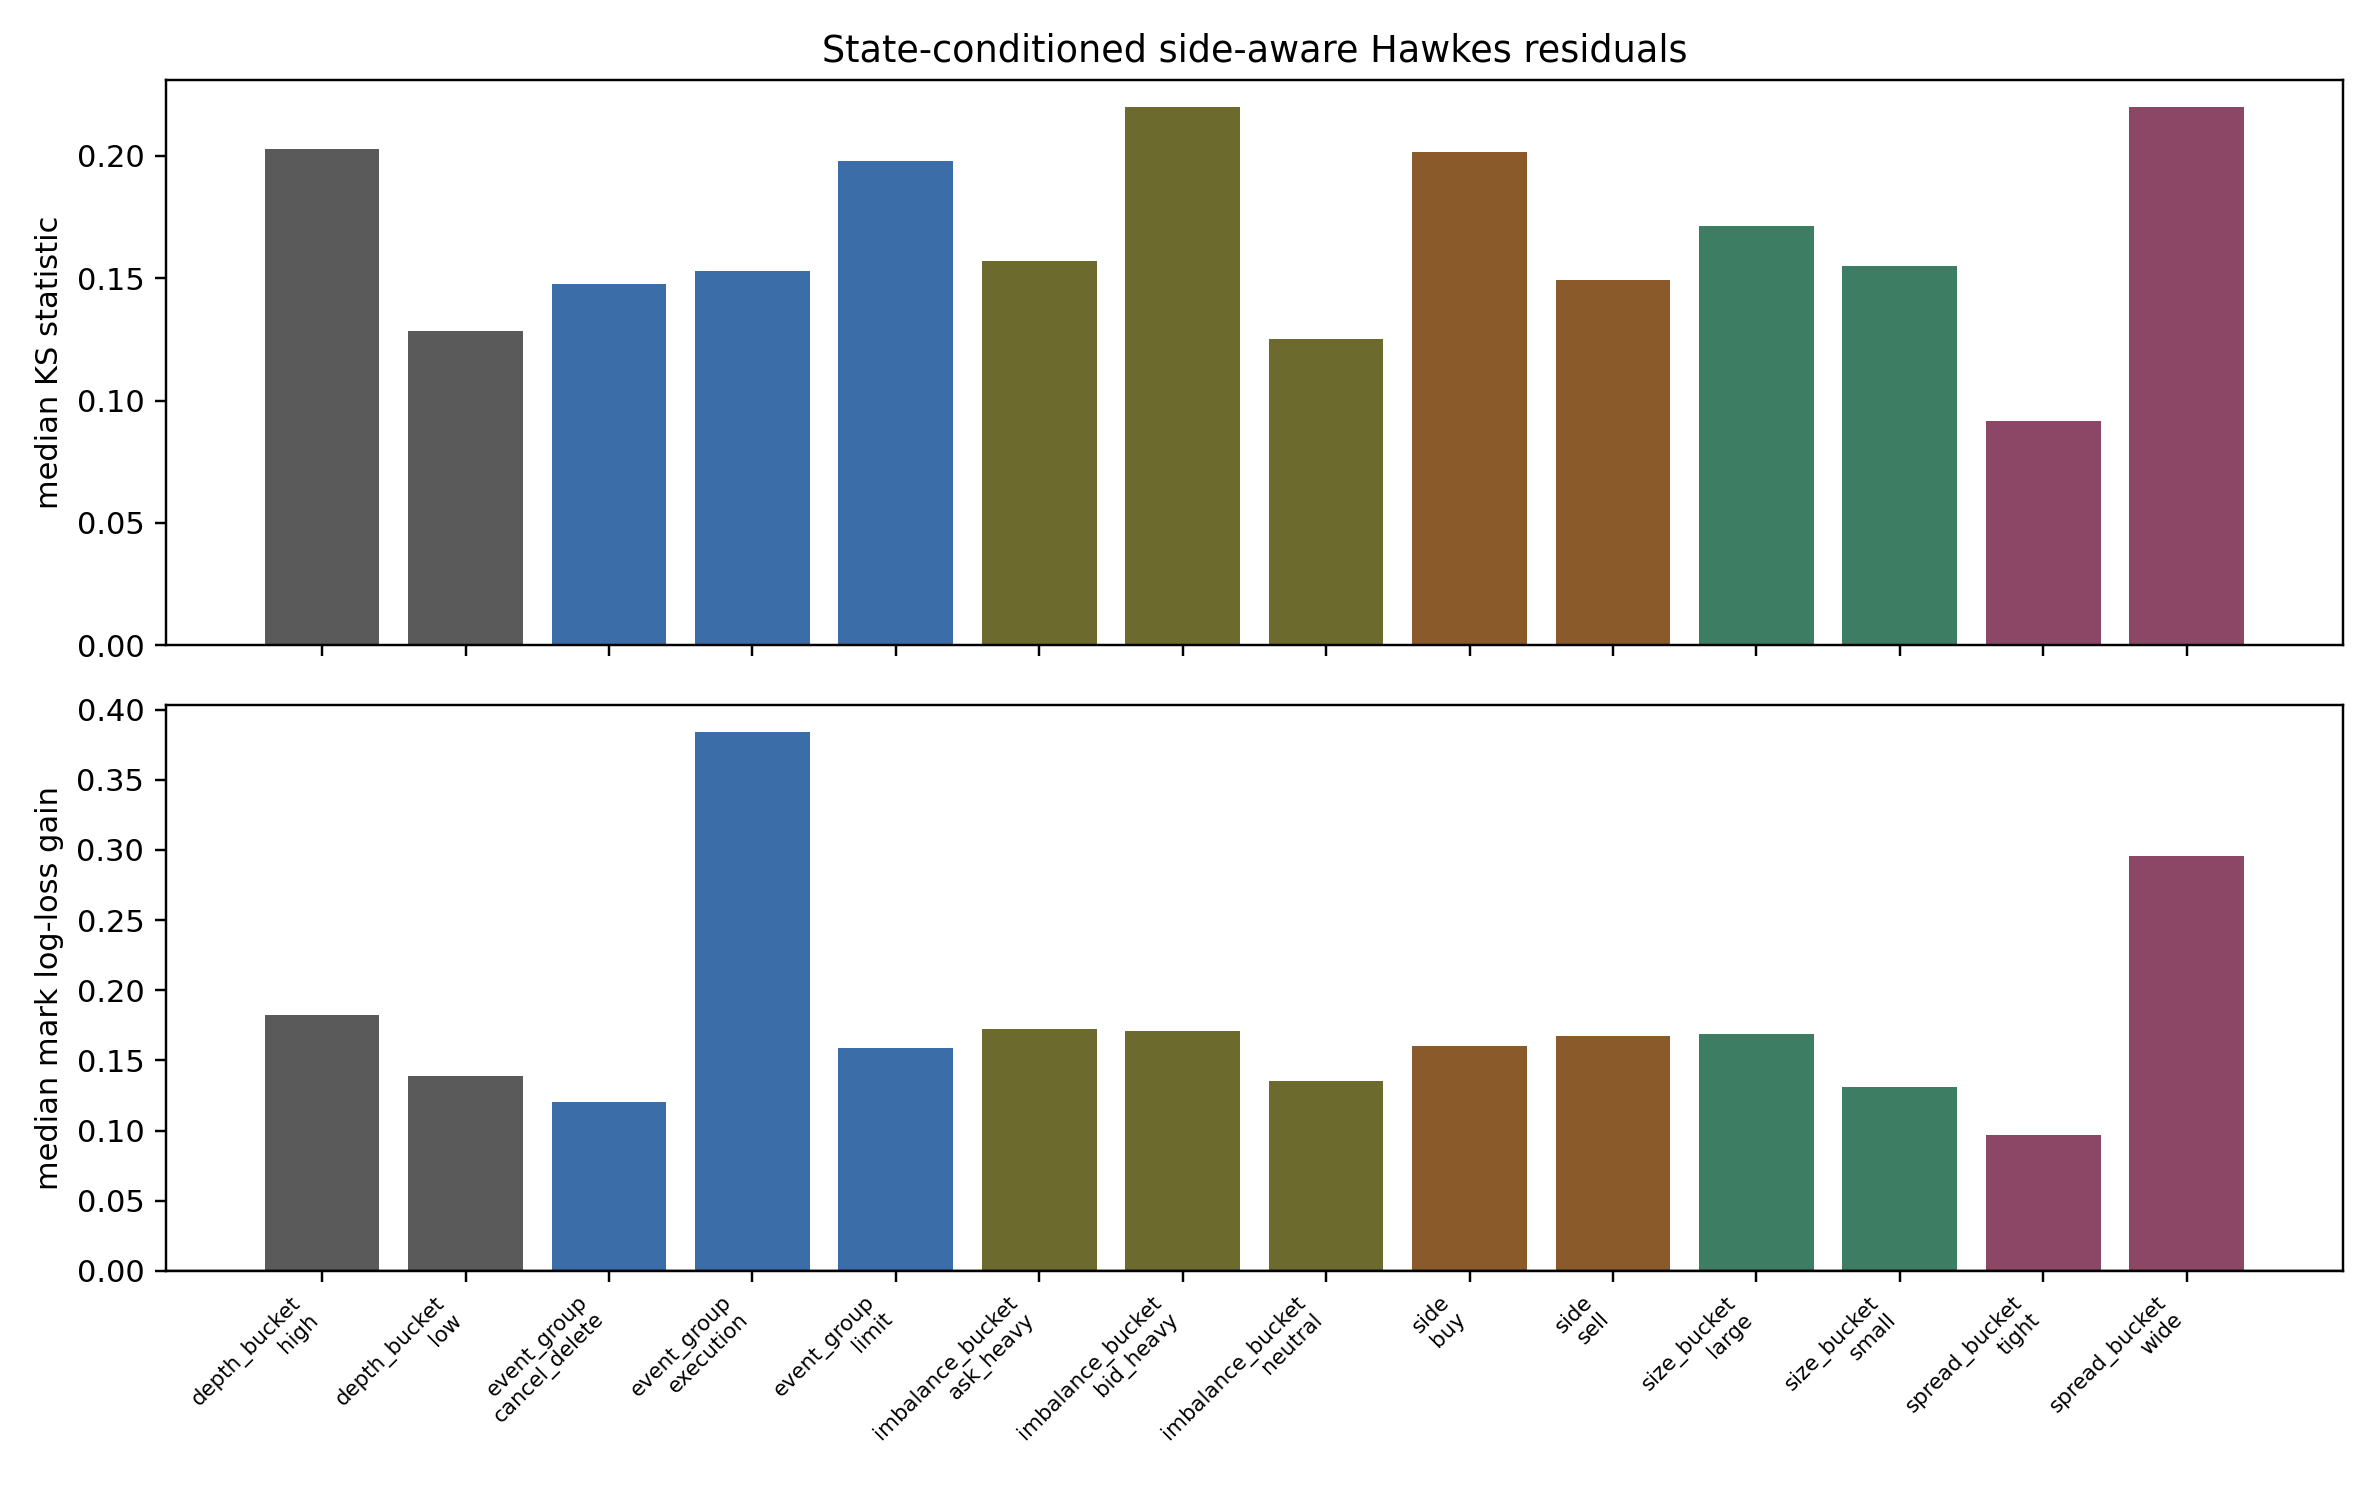
\includegraphics[width=.86\linewidth]{../results/figures/lobster_side_marked_state_residuals.png}
\caption{State-conditioned residual diagnostics for the side-aware six-mark
Hawkes fit. Residual deviations and mark-prediction gains vary by spread,
depth, imbalance, and event-size bucket, so the public-data calibration should
be treated as a diagnostic input rather than a complete structural law.}
\end{figure}

\section{Scope Conditions And Extensions}

The current package gives a conditional multitype HJBI control bridge for the
stated exponential Hawkes model class. The proof layers are compact truncated
HJBI verification under compact-PDMP DPP/comparison hypotheses, untruncated
Lyapunov stability with $p>1$ tail control, pairwise weighted comparison and
uniqueness in fixed-boundary $W_v$-weighted subclasses, local differentiability
of smooth interior quote optimizers, and an assembled end-to-end theorem
combining these layers. It does not claim the same theorem for every
possible state dependent, learned, multiscale, or power law Hawkes kernel
without rechecking the stated Lyapunov and comparison assumptions. It also
treats no-quote and active adversary switches as nonsmooth control boundaries
rather than classical optimizer derivatives.

The current top-of-book, L1, displayed-depth, residual-volume priority-aware
level-10, deepest-public level-50, priority-sensitivity, and
observable-reconstruction LOBSTER audits should still be treated as public-data
execution audits rather than production execution claims, because hidden
liquidity and anonymous initial queue priority remain unobserved. Binance
aggregate trades should remain event-clustering evidence rather than a
queue-calibration source. These scope conditions discipline the paper around
its correct novelty: structural Hawkes ambiguity, criticality amplification,
and calibration fragility in Hawkes market-making experiments.

\section*{Acknowledgments}

Portions of the manuscript drafting, code scaffolding, experiment automation,
documentation, and validation scripts were prepared with assistance from
OpenAI Codex, a GPT-5 based coding assistant, on May 16, 2026. The human
authors are responsible for all mathematical claims, proofs, citations, code,
data processing, numerical experiments, and final text included in the
submitted manuscript.

\begin{thebibliography}{99}
\bibitem{BacryMuzy2015} E. Bacry, I. Mastromatteo, and J.-F. Muzy. Hawkes
processes in finance. arXiv:1502.04592, 2015.
\bibitem{LawViens2019} B. Law and F. Viens. Market making under a weakly
consistent limit order book model. arXiv:1903.07222, 2019.
\bibitem{Kumar2024} P. Kumar. Deep Hawkes Process for High-Frequency Market
Making. Journal of Banking and Financial Technology, 2024. arXiv:2109.15110,
doi:10.1007/s42786-024-00049-8.
\bibitem{Raffaelli2026} D. Raffaelli, R. G. Cestari, D. Marazzina, and
S. Formentin. Forecasting Bitcoin price movements using multivariate Hawkes
processes and limit order book data. Decisions in Economics and Finance, 2026.
doi:10.1007/s10203-026-00570-z.
\bibitem{WangNoQuote2025} Z. Wang, C. Ventre, and M. Polukarov. Robust
Market Making: To Quote, or not To Quote. arXiv:2508.16588, 2025.
\bibitem{WangHawkesARL2025} Z. Wang, C. Ventre, and M. Polukarov. ARL-Based
Multi-Action Market Making with Hawkes Processes and Variable Volatility.
arXiv:2508.16589, 2025.
\bibitem{LalorSwishchuk2025} L. Lalor and A. Swishchuk. Event-Based Limit
Order Book Simulation under a Neural Hawkes Process: Application in
Market-Making. arXiv:2502.17417, 2025.
\bibitem{GuoAttnLOB2023} X. Guo, H. Lin, and T. Huang. Market Making with
Deep Reinforcement Learning from Limit Order Books. arXiv:2305.15821, 2023.
\bibitem{Jiang2025} J. Jiang, C. Yang, X. Wang, Z. Li, X. Huang, and B. Li.
Resolving Latency and Inventory Risk in Market Making with Reinforcement
Learning. arXiv:2505.12465, 2025.
\bibitem{Jain2025} S. Jain, N. Firoozye, J. Kochems, and P. Treleaven. An
Impulse Control Approach to Market Making in a Hawkes LOB Market.
arXiv:2510.26438, 2025.
\bibitem{ElKarmiSimulator2025} S. El Karmi. A Deterministic Limit Order Book
Simulator with Hawkes-Driven Order Flow. arXiv:2510.08085, 2025.
\bibitem{Noble2026} P. Noble, M. Rosenbaum, and S. Souilmi. Bridging the
Reality Gap in Limit Order Book Simulation. arXiv:2603.24137, 2026.
\bibitem{Kimura2026} A. Kimura. Extended State-dependent Hawkes Process for
Limit Order Books: Mathematical Foundation and the Reproduction of Volatility
Signature Plots. arXiv:2604.23961, 2026.
\bibitem{SzymanskiXu2025} G. Szymanski and Y. Xu. Mean-Field Limits for
Nearly Unstable Hawkes Processes. arXiv:2501.11648, 2025.
\bibitem{ElKarmi2026} S. El Karmi. Scaling Limits of Bivariate
Nearly-Unstable Hawkes Processes and Applications to Rough Volatility.
arXiv:2605.03703, 2026.
\bibitem{Hardiman2013} S. Hardiman, N. Bercot, and J.-P. Bouchaud. Critical
reflexivity in financial markets. arXiv:1302.1405, 2013.
\bibitem{Kang2026} S. Kang. The Physics of Price Discovery. arXiv:2601.11602,
2026.
\bibitem{Ogata1988} Y. Ogata. Statistical models for earthquake occurrences
and residual analysis for point processes. Journal of the American Statistical
Association, 83(401):9--27, 1988.
\url{https://doi.org/10.1080/01621459.1988.10478560}.
\end{thebibliography}

\end{document}
